\documentclass{article}

% Language setting
% Replace `english' with e.g. `spanish' to change the document language
\usepackage[english]{babel}
\usepackage{caption}
\usepackage{subcaption}
\newcommand{\Rho}{\mathrm{P}}

\newtheorem{theorem}{Theorem}
\newtheorem{proposition}{Proposition}

% Set page size and margins
% Replace `letterpaper' with`a4paper' for UK/EU standard size
\usepackage[letterpaper,top=2cm,bottom=2cm,left=3cm,right=3cm,marginparwidth=1.75cm]{geometry}

% Useful packages
\usepackage{amsmath}
\usepackage{tabularx}
\usepackage{amsfonts}
\usepackage{graphicx}
\usepackage{siunitx}
\usepackage{float}
\usepackage[colorlinks=true, allcolors=blue]{hyperref}
\usepackage{bbm}
\usepackage[scr=rsfso]{mathalfa}
\usepackage{amssymb}
\usepackage{xcolor}
\usepackage{minted}
\usepackage{sourcecodepro}

\setminted{fontsize=\footnotesize}

\title{ELEC 844 Assignment 2}
\author{Ilir Gusija}
\date{\today}

\begin{document}

\begin{titlepage}
\maketitle
\begin{center}
    \textbf{Presented to:}\\
    Prof. Jonathan Gammell\\
    \vspace{5mm}

    Assignment 2\\
    ELEC 844\\
    Electrical and Computer Engineering\\
    Queen's University\\
    \vspace{5mm}
    
\end{center}
\end{titlepage}

\section{Probabilistically Complete Samping-based Planning}
\subsection{Data and Figures}\label{sub:Data and Figures} % (fold)
\begin{table}[h!]
    \centering
    \begin{tabularx}{\textwidth}{|c|X|X|X|}
        \hline
        \multicolumn{4}{|c|}{\textbf{Table 1: Results of RRT from 100 trials}} \\ \hline
        \textbf{Value of} $\ell$ & 
        \textbf{Median \# of iterations} & 
        \textbf{Median \# of vertices} & 
        \textbf{Median path length} \\ \hline
        25 & 448.5 & 377.0 & 105.45 \\ \hline
        4  & 1395.0 & 798.0 & 155.05 \\ \hline
    \end{tabularx}
\end{table}

Included below are the visualizations of the paths taken by RRT. 
\begin{itemize}
    \item $\mathbb{S},\mathbb{G}$ represent the start and end respectively. 
    \item Yellow edges represent the expanded nodes. 
    \item Red edges represent the final solution. 
    \item The blue rectangle represents the obstacle
\end{itemize}
\begin{figure}[H]
    \begin{center}
        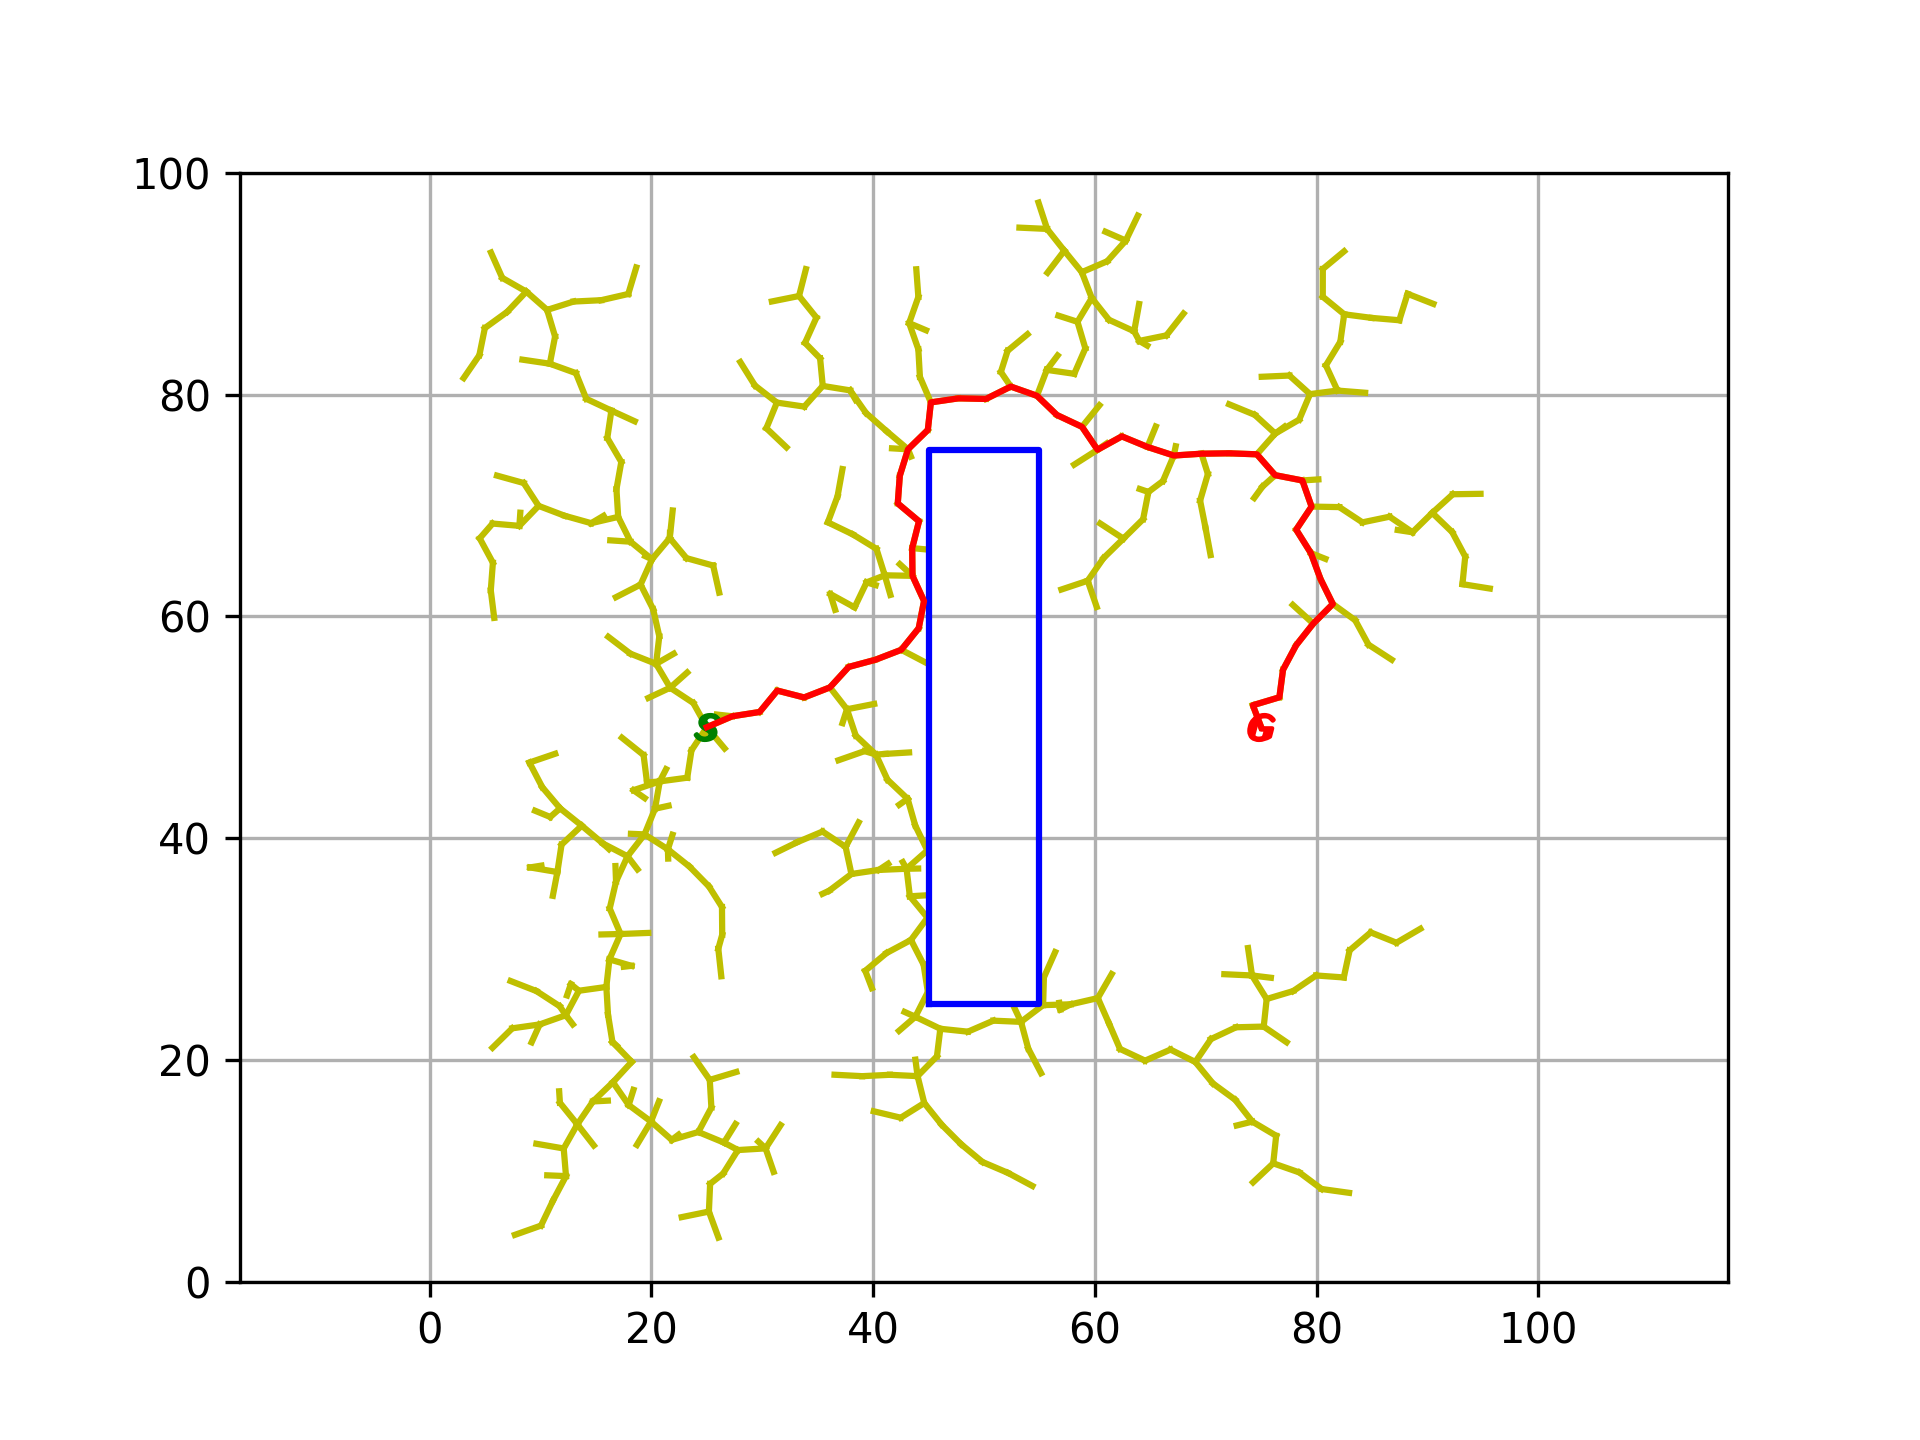
\includegraphics[width=0.45\textwidth]{figures/final_path_RRT_1.png}
    \end{center}
    \caption{Example of RRT on map with $\ell=25$}\label{fig:RRT_1}
\end{figure}
\begin{figure}[H]
    \begin{center}
        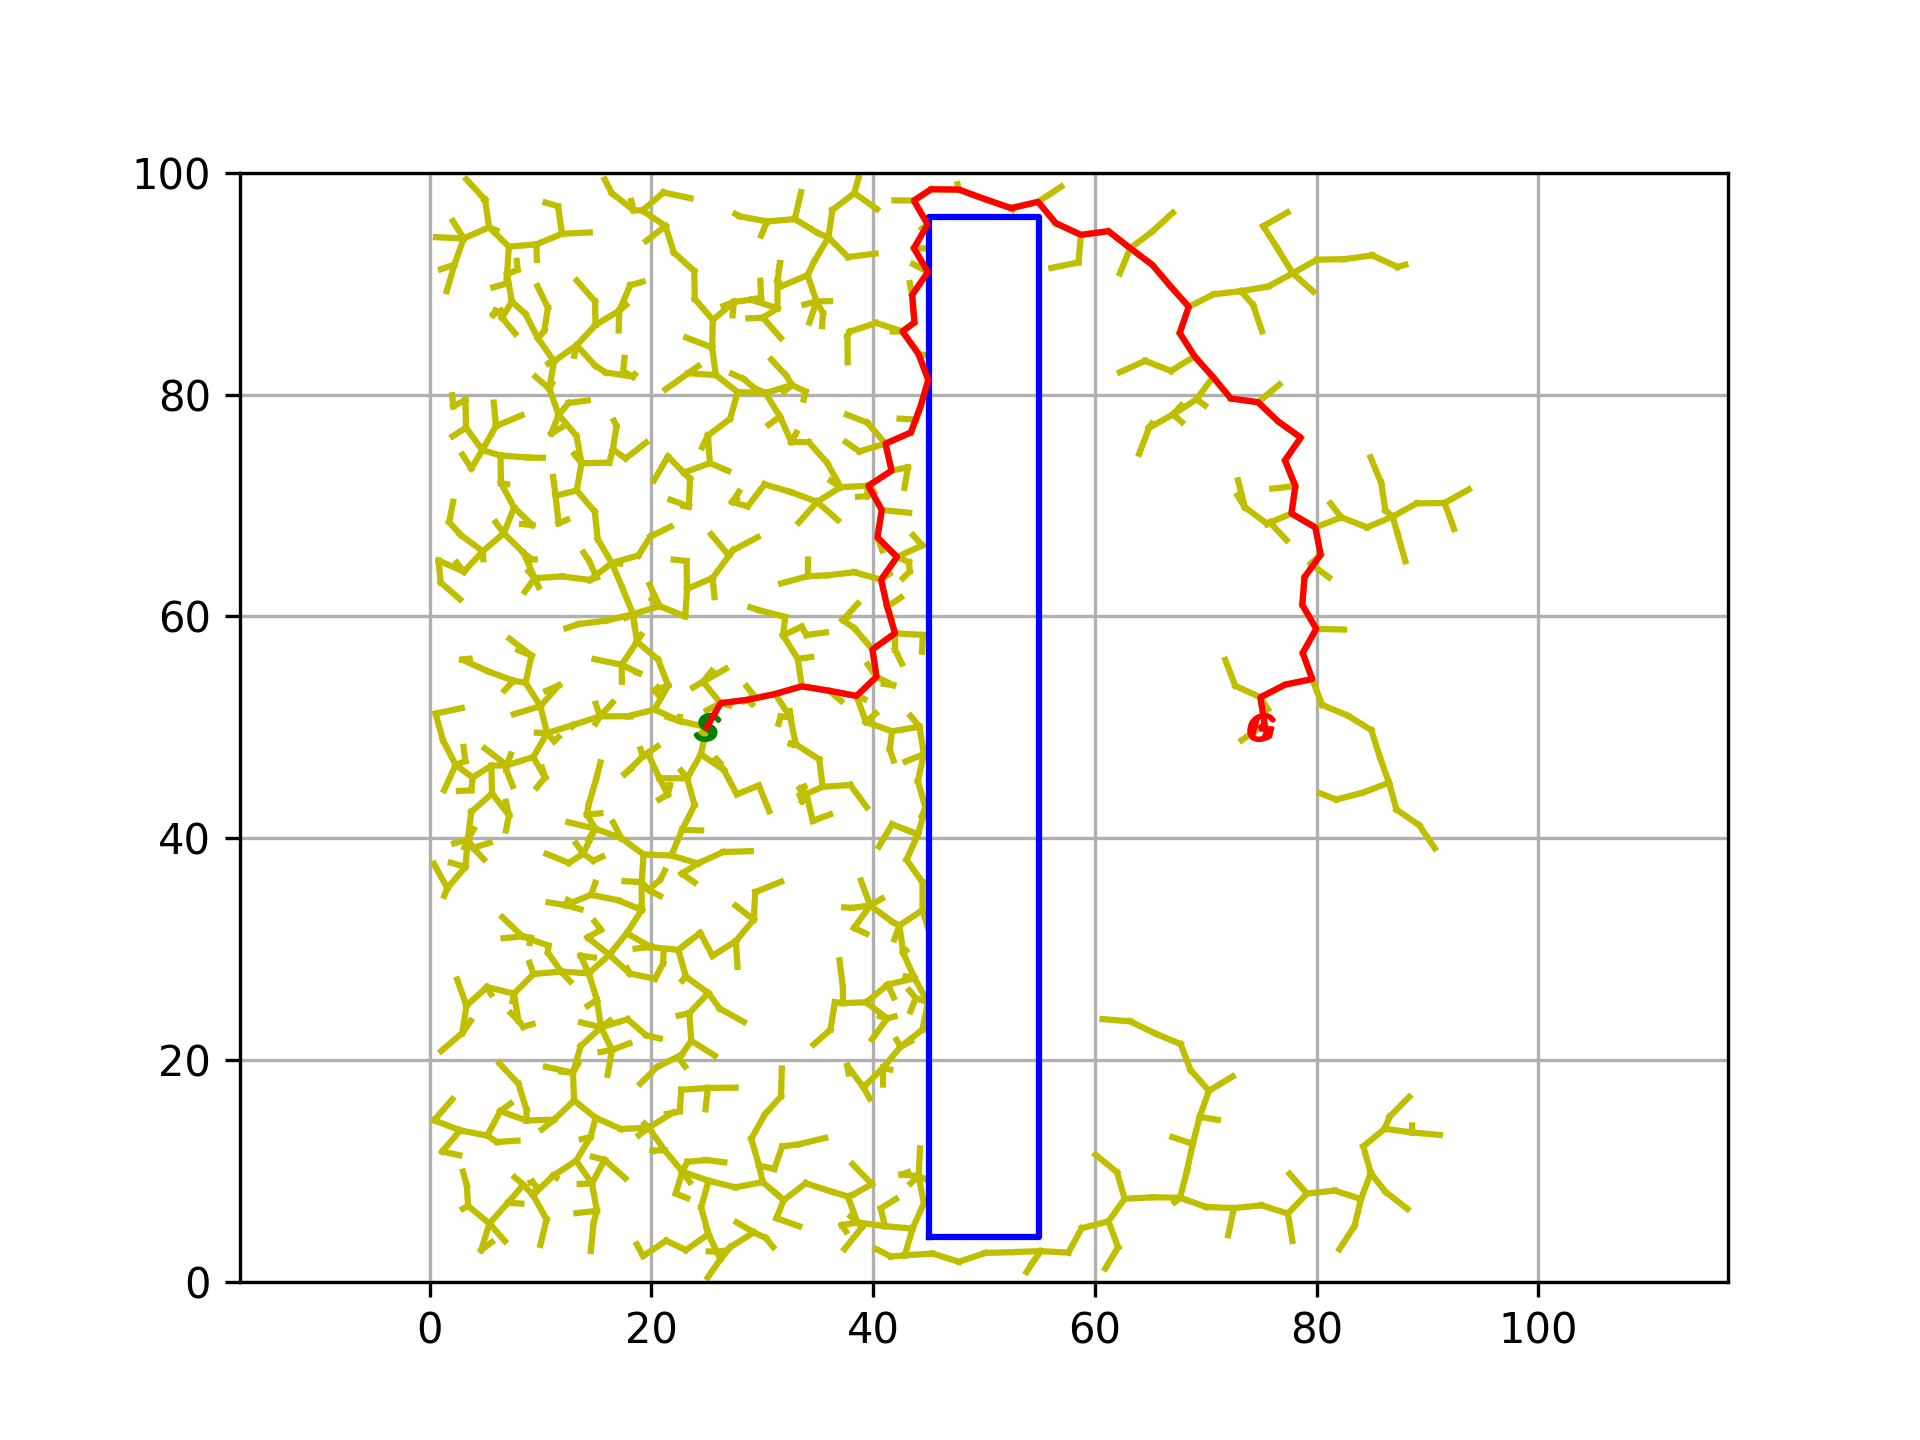
\includegraphics[width=0.45\textwidth]{figures/final_path_RRT_2.png}
    \end{center}
    \caption{Example of RRT on map with $\ell=4$}\label{fig:RRT_2}
\end{figure}
and some histograms depicting the number of iterations and vertices for each trial
\begin{figure}[H]
    \begin{center}
        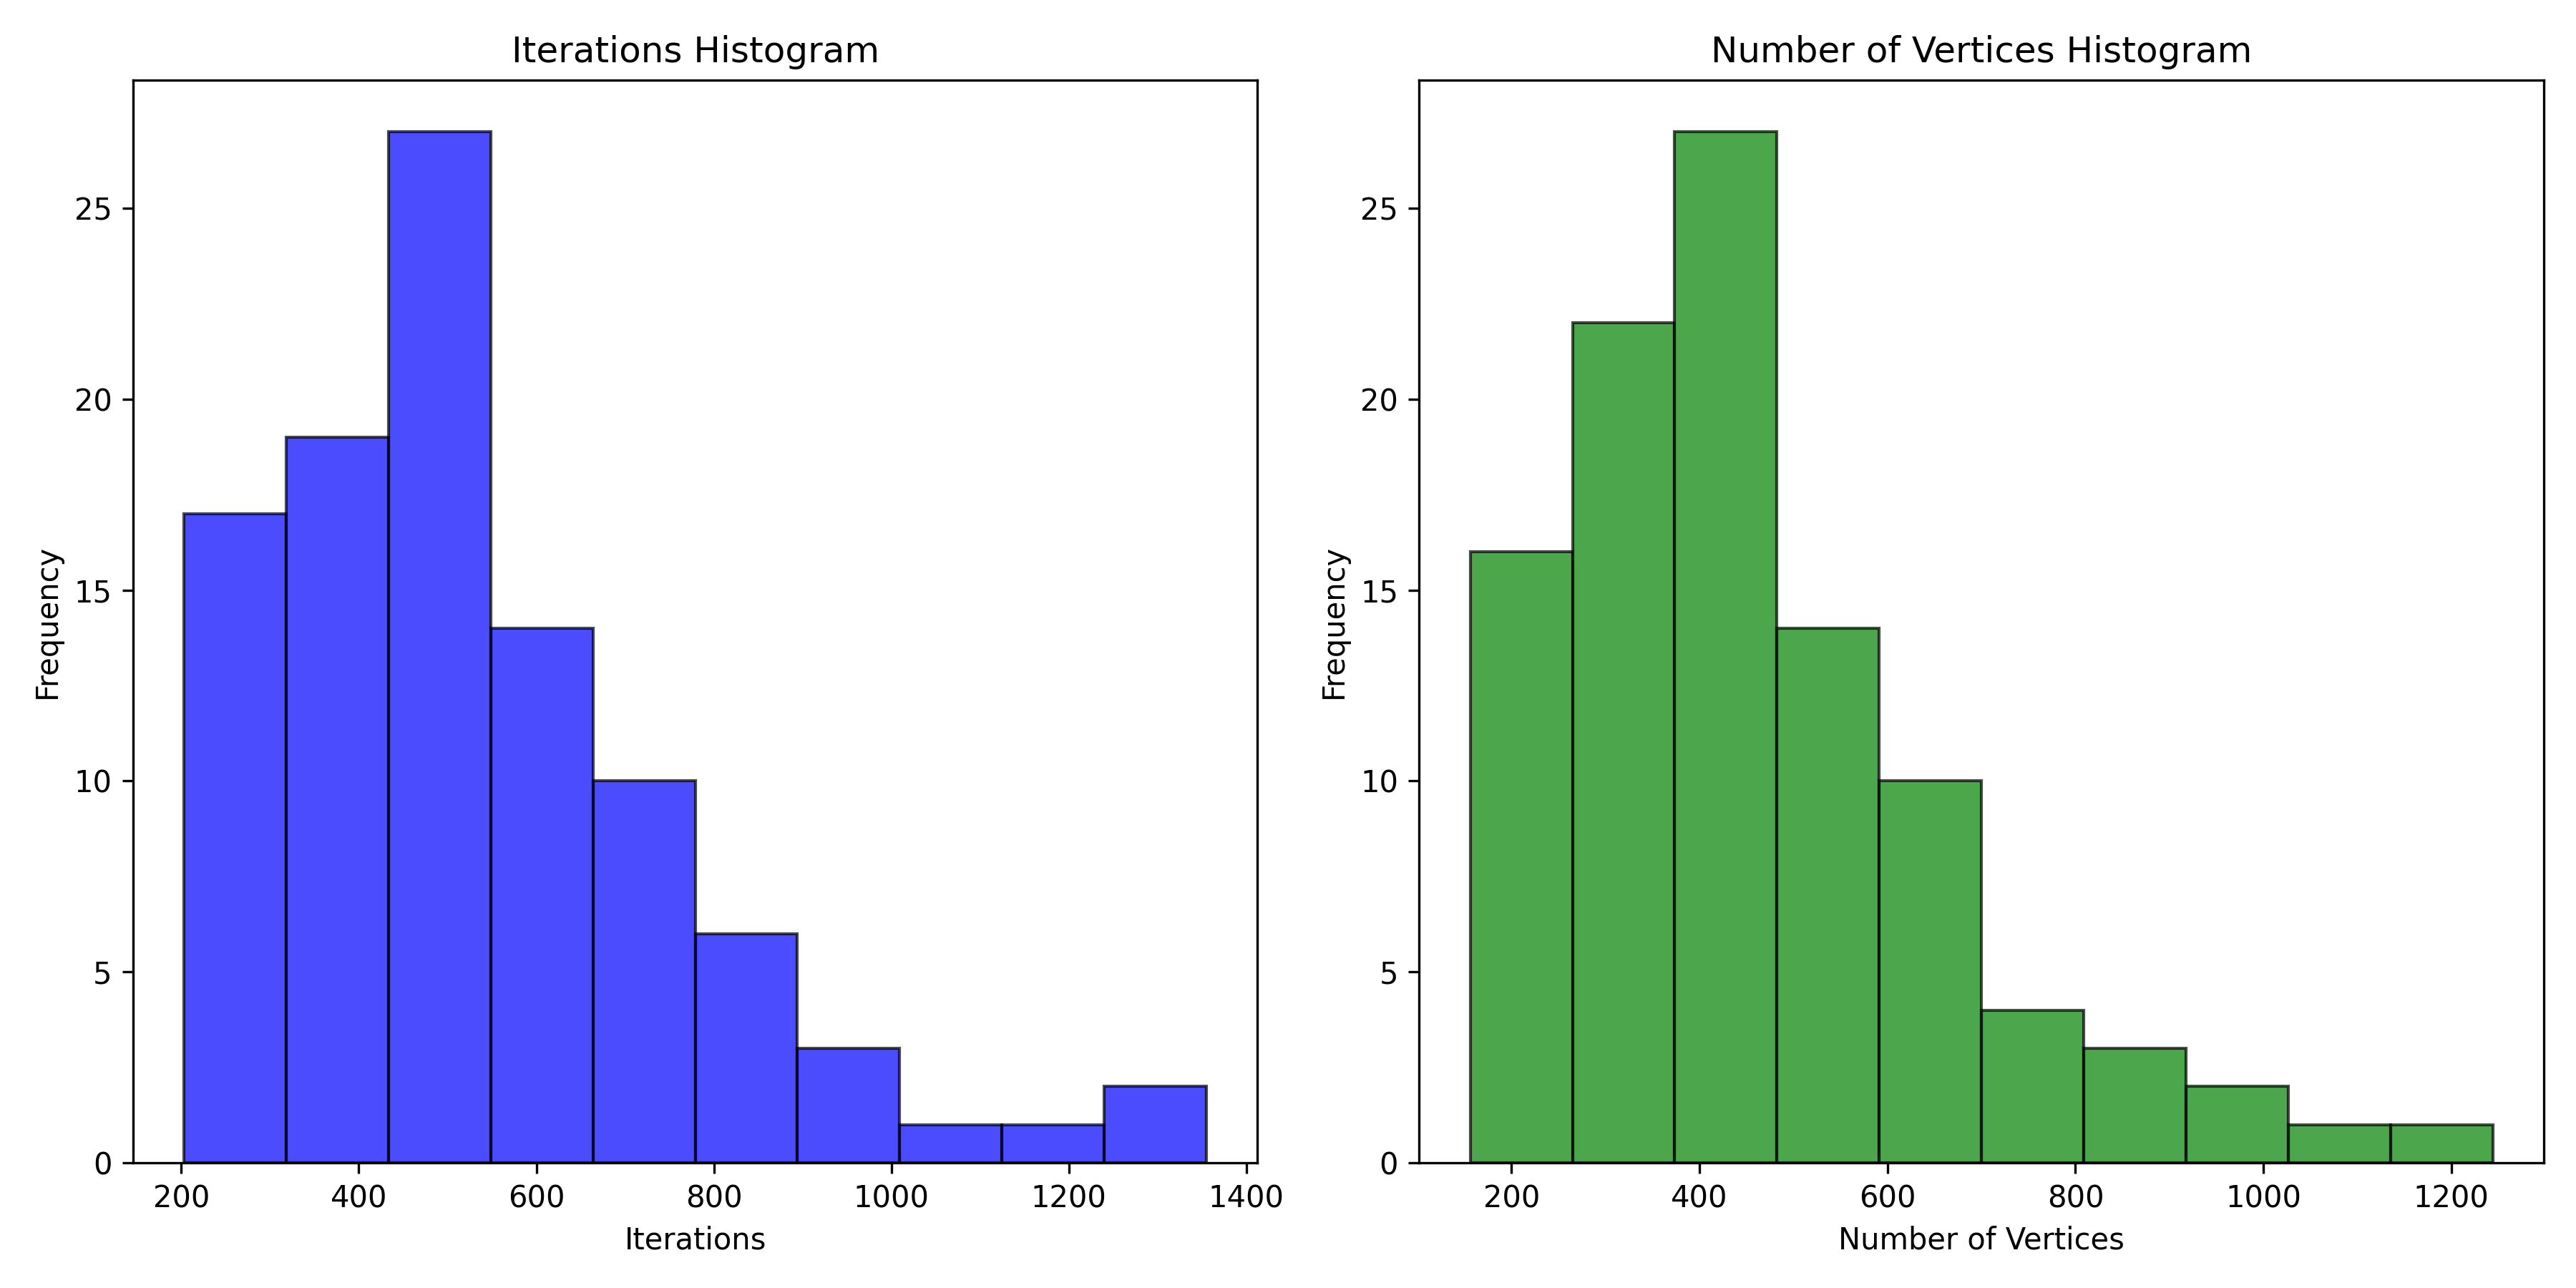
\includegraphics[width=0.65\textwidth]{figures/hist_RRT_1.png}
    \end{center}
    \caption{Histogram depicting number of iterations and number of
    vertices of RRT on map with $\ell=25$ over 100
trials}\label{fig:hist_RRT_1}
\end{figure}
\begin{figure}[H]
    \begin{center}
        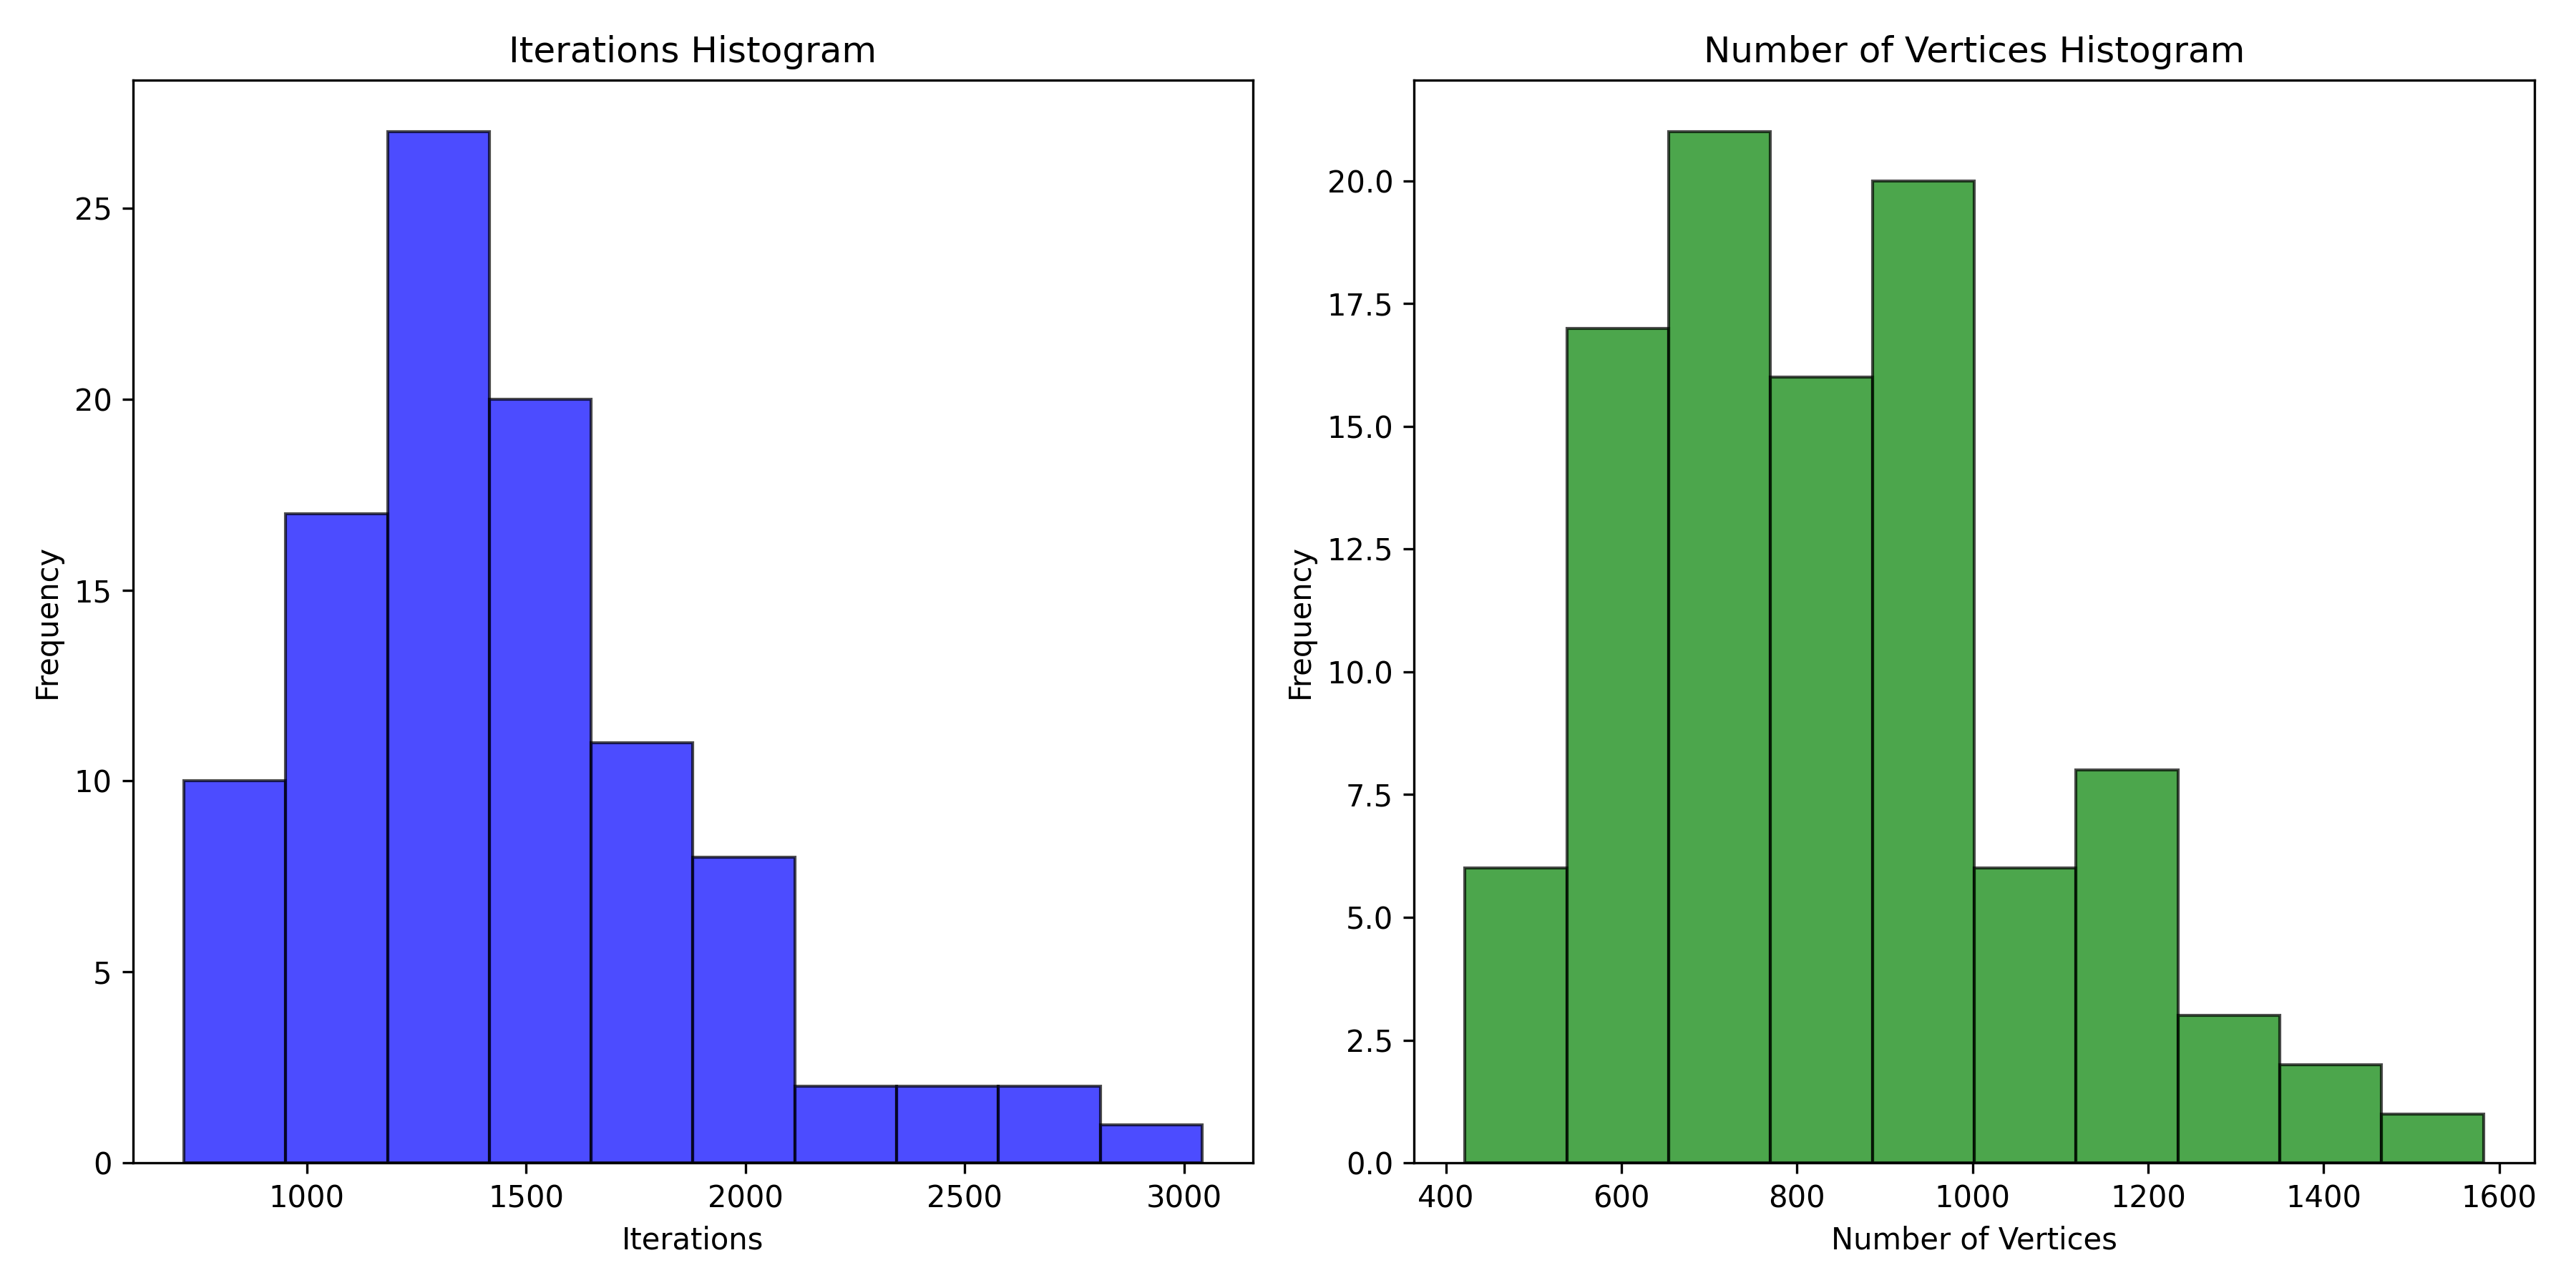
\includegraphics[width=0.65\textwidth]{figures/hist_RRT_2.png}
    \end{center}
    \caption{Histogram depicting number of iterations and number of
    vertices of RRT on map with $\ell=4$ over 100
trials}\label{fig:hist_RRT_2}
\end{figure}
% subsection Data and Figures (end)

\subsection{Discussion}\label{sub:Discussion} % (fold)
We clearly see that increasing the size of the obstacle increases the
computational effort of the algorithm. The ratio of vertices to iterations
when $\ell=25$ amounts to $0.84$ and in the case of the larger obstacle
$\ell=4$ we get $0.57$ indicating our algorithm has a greater percentage
of failed iterations (failed in the sense that we haven't expanded any
additional vertices). Moving our discussion to the histograms we also see the 
absolute amount of iterations experiences a large increase while the absolute 
amount of vertices experiences a modest increase.
% subsection Discussion (end)

\subsection{Code}\label{sub:Code} % (fold)
\subsubsection{RRT.py}
\begin{minted}{python}
import math
import random
from itertools import count

import matplotlib.pyplot as plt

class Vertex:
    def __init__(self, x, y):
        self.x = x
        self.y = y
        self.path_x = []
        self.path_y = []
        self.parent = None
    def __eq__(self, other):
        if isinstance(other, Vertex):
            return self.x == other.x and self.y == other.y
        return False
    def __hash__(self):
        return hash((self.x, self.y))

class RRT:
    def __init__(self, start, goal, obstacle, workspace, animation=True, eta=2.5,
                 goal_sample_rate=0.01):
        """
        start:Start Position [x,y]
        goal:Goal Position [x,y]
        obstacle:Coordinates of rectangle obstacle [left,right,bottom,top]
        workspace:Min/max coordinates of our square arena [min,max]
        """
        self.start = Vertex(start[0], start[1])
        self.goal = Vertex(goal[0], goal[1])
        self.min_rand = workspace[0]
        self.max_rand = workspace[1]
        self.eta = eta
        self.goal_sample_rate = goal_sample_rate
        self.animation=animation
        self.obstacle = []
        if isinstance(obstacle, tuple):
            self.obstacle.append(self.convert_to_rectangle(obstacle[0],obstacle[1],self.min_rand,self.max_rand)) 
        elif isinstance(obstacle, list):
            for o in obstacle:
                ref, length, orientation, translation = o
                self.obstacle.append(self.generate_rectangle_from_reference(ref, length, orientation, translation))
        self.vertices = []
        self.iterations = 0
        self.num_vertices = 0

    def planning(self):
        self.vertices = [self.start]
        for self.iterations in count(): 
            if self.goal in self.vertices:
                break
            x_rand = self.sample_random_vertex()
            v_nearest = self.get_nearest_vertex(x_rand, self.vertices)
            x_new = self.steer(v_nearest, x_rand)

            if self.is_edge_valid(v_nearest, x_new):
                self.vertices.append(x_new)

            if self.iterations % 3 and self.animation is True == 0:
                self.update_graph(x_rand)

        return self.final_path(len(self.vertices) - 1)

    def steer(self, v_nearest, x_rand):
        x_new = Vertex(v_nearest.x, v_nearest.y)
        d, angle = self.calc_distance_and_angle(x_new, x_rand)

        x_new.path_x = [x_new.x]
        x_new.path_y = [x_new.y]

        if self.eta < d:
            x_new.x += self.eta * math.cos(angle)
            x_new.y += self.eta * math.sin(angle)
        else:
            x_new.x += d * math.cos(angle)
            x_new.y += d * math.sin(angle)

        x_new.path_x.append(x_new.x)
        x_new.path_y.append(x_new.y)

        x_new.parent = v_nearest 

        return x_new

    def is_vertex_valid(self, vertex):
        if vertex is None:
            return False
        for o in self.obstacle:
            left, right, bottom, top = o
            for x, y in zip(vertex.path_x, vertex.path_y):
                if (left  <= x <= right and bottom <= y <= top):
                    return False  
        return True  

    def is_edge_valid(self, v_nearest, x_rand):
        path_resolution=0.1
        x_new = Vertex(v_nearest.x, v_nearest.y)
        d, angle = self.calc_distance_and_angle(x_new, x_rand)
        if not self.is_vertex_valid(x_rand):
            return False
        x_new.path_x = [x_new.x]
        x_new.path_y = [x_new.y]

        if self.eta > d:
            n_steps = math.floor(d / path_resolution)
        else:
            n_steps = math.floor(self.eta / path_resolution)

        for _ in range(n_steps):
            x_new.x += path_resolution * math.cos(angle)
            x_new.y += path_resolution * math.sin(angle)
            if not self.is_vertex_valid(x_new):
                return False
            x_new.path_x.append(x_new.x)
            x_new.path_y.append(x_new.y)

        d, _ = self.calc_distance_and_angle(x_new, x_rand)
        if d <= path_resolution:
            x_new.path_x.append(x_rand.x)
            x_new.path_y.append(x_rand.y)
            x_new.x = x_rand.x
            x_new.y = x_rand.y

        return True

    def update_graph(self, sampled_vec=None):
        plt.clf()
        # Plot the sampled vector as a black plus sign
        if sampled_vec is not None:
            plt.plot(sampled_vec.x, sampled_vec.y, "Pk")

        # Plot edges as yellow lines
        for vertex in self.vertices:
            if vertex.parent:
                plt.plot(vertex.path_x, vertex.path_y, "-y")

        for o in self.obstacle:
            # Plot the blue rectangle obstacle
            self.plot_rectangle(o)

        # Plot the green start "S" and red goal "G"
        plt.plot(self.start.x, self.start.y, c="g", marker=r"$\mathbb{S}$")
        plt.plot(self.goal.x, self.goal.y, c="r", marker=r"$\mathbb{G}$")

        plt.axis("equal")
        plt.axis([self.min_rand, self.max_rand, self.min_rand, self.max_rand])
        plt.grid(True)
        plt.pause(0.01)

    def sample_random_vertex(self):
        if random.random() <= self.goal_sample_rate:
            sampled_vec = Vertex(self.goal.x, self.goal.y)
        else: 
            while True:
                sampled_vec = Vertex(random.uniform(self.min_rand, self.max_rand),
                    random.uniform(self.min_rand, self.max_rand))
                if self.is_vertex_valid(sampled_vec) is True:
                    break
        return sampled_vec

    def get_nearest_vertex(self, x_rand, vertices):
        dlist = [self.L2_norm(vertex, x_rand) for vertex in vertices]
        minind = dlist.index(min(dlist))
        return vertices[minind]

    def final_path(self, g_idx):
        path = [[self.goal.x, self.goal.y]]
        vertex = self.vertices[g_idx]
        while vertex.parent is not None:
            path.append([vertex.x, vertex.y])
            vertex = vertex.parent
        path.append([vertex.x, vertex.y])
        self.num_vertices = len(self.vertices)
        return path

    @staticmethod
    def L2_norm(left, right):
        return (left.x - right.x)**2 + (left.y - right.y)**2

    @staticmethod
    def convert_to_rectangle(l, width, min_rand, max_rand):
        map_width = max_rand - min_rand  # Assuming square map

        # Calculate the top, bottom, left, and right boundaries of the rectangle
        top = max_rand - l
        bottom = l
        left = (map_width - width) / 2
        right = left + width

        # Check for valid rectangle within map bounds
        if bottom < min_rand or top > max_rand or width > map_width:
            raise ValueError("Invalid rectangle dimensions: exceeds map bounds.")

        return left, right, bottom, top

    @staticmethod
    def plot_rectangle(rectangle, color="-b"):
        left, right, bottom, top = rectangle

        # Rectangle corners
        x_coords = [left, right, right, left, left]
        y_coords = [bottom, bottom, top, top, bottom]

        # Plot the rectangle
        plt.plot(x_coords, y_coords, color)

    @staticmethod
    def calc_distance_and_angle(parent, child):
        dx = child.x - parent.x
        dy = child.y - parent.y
        length = math.hypot(dx, dy)
        angle = math.atan2(dy, dx)
        return length, angle

    @staticmethod
    def generate_rectangle_from_reference(reference, length, orientation="horizontal", translation=(10, 0)):
        x_ref, y_ref = reference
        dx, dy = translation
        x_translated = x_ref + dx
        y_translated = y_ref + dy

        if orientation == "horizontal":
            # Fixed height of 10, horizontal length is variable
            left = x_translated-length/2
            right = x_translated + length/2
            bottom = y_translated - 2.5
            top = y_translated + 2.5
        elif orientation == "vertical":
            # Fixed width of 10, vertical length is variable
            left = x_translated - 2.5
            right = x_translated + 2.5
            bottom = y_translated-length/2
            top = y_translated + length/2
        else:
            raise ValueError("Invalid orientation. Choose 'horizontal' or 'vertical'.")

        return left, right, bottom, top
\end{minted}
\subsubsection{main.py}
\begin{minted}{python}
import argparse
import matplotlib.pyplot as plt
import numpy as np
import pandas as pd

from RRT import RRT
from RRT_Connect import RRT_Connect

import math

def compute_path_length(path):
    if len(path) < 2:
        return 0  

    total_length = 0.0
    for i in range(1, len(path)):
        x1, y1 = path[i-1]
        x2, y2 = path[i]
        distance = math.sqrt((x2 - x1)**2 + (y2 - y1)**2)
        total_length += distance

    return total_length

def select_planner(alg, start, goal, obstacle, animation):
    rrt=None
    if alg == "RRT":
        rrt = RRT(
            start=start,
            goal=goal,
            workspace=[0, 100],
            obstacle=obstacle,
            animation=animation
        )
    elif alg == "RRT_Connect":
        rrt = RRT_Connect(
            start=start,
            goal=goal,
            workspace=[0, 100],
            obstacle=obstacle,
            animation=animation
        )
    return rrt

def histograms(alg, obs, iterations, num_verts):
    plt.figure(figsize=(12, 6))

    plt.subplot(1, 2, 1)
    plt.hist(iterations, bins=10, color='blue', alpha=0.7, edgecolor='black')
    plt.title("Iterations Histogram")
    plt.xlabel("Iterations")
    plt.ylabel("Frequency")

    plt.subplot(1, 2, 2)
    plt.hist(num_verts, bins=10, color='green', alpha=0.7, edgecolor='black')
    plt.title("Number of Vertices Histogram")
    plt.xlabel("Number of Vertices")
    plt.ylabel("Frequency")

    plt.tight_layout()
    plt.savefig(f"figures/hist_{alg}_{obs}.png", format="png", dpi=300)

def save_medians_to_csv(iterations, num_verts, paths, alg, obs, csv_file="results.csv"):
    median_iterations = np.median(iterations)
    median_num_verts = np.median(num_verts)
    median_paths = np.median(paths)

    column_name = f"{alg}_{obs}"

    try:
        df = pd.read_csv(csv_file, index_col=0)
    except FileNotFoundError:
        df = pd.DataFrame(index=["iterations", "num_verts", "paths"])

    df[column_name] = [median_iterations, median_num_verts, median_paths]

    df.to_csv(csv_file)

def main(obs, alg, animation):
    start=[25.0, 50.0]
    goal=[75.0, 50.0]
    # Define obstacles
    bug_trap_start = [[start, 30, "vertical", (12.5,0)], 
                 [start, 20, "horizontal", (0, -12.5)],
                 [start, 20, "horizontal", (0,12.5)],
                 [start, 14, "vertical", (-12.5,8)],
                 [start, 14, "vertical", (-12.5,-8)] ]
    bug_trap_goal = [[goal, 30, "vertical", (-12.5,0)], 
                 [goal, 20, "horizontal", (0, -12.5)],
                 [goal, 20, "horizontal", (0,12.5)],
                 [goal, 14, "vertical", (12.5,8)],
                 [goal, 14, "vertical", (12.5,-8)] ]
    obstacles = [(25, 10), (4, 10), bug_trap_start, bug_trap_goal,
                 bug_trap_start + bug_trap_goal]
    obstacle = obstacles[obs-1]

    # Run the selected algorithm
    path = []
    planners=[]
    num_iters=1
    for i in range(0,num_iters):
        print(f"Iteration: {i}")
        if i==num_iters-1:
            planners.append(select_planner(alg, start, goal, obstacle, True)) 
        else:
            planners.append(select_planner(alg, start, goal, obstacle, animation)) 

        path.append(planners[i].planning())

        if planners[i].animation is True:
            planners[i].update_graph()
            plt.plot([x for (x, _) in path[i]], [y for (_, y) in path[i]], '-r')
            plt.grid(True)
            plt.pause(0.01)
            plt.savefig(f"figures/final_path_{alg}_{obs}.png", format="png", dpi=300)

    if num_iters >= 100:
        iterations = [planner.iterations for planner in planners]
        num_verts = [planner.num_vertices for planner in planners]
        histograms(alg, obs, iterations, num_verts)
        save_medians_to_csv(iterations, num_verts, [compute_path_length(p) for p in path], alg, obs)

if __name__ == '__main__':
    parser = argparse.ArgumentParser(description="Run specific RRT algorithms with selected obstacles.")
    parser.add_argument(
        "--animation",
        type=str,
        choices=["t","f"],
        default="t",
        help="Select True or False for animation"
    )
    parser.add_argument(
        "--obstacle", 
        type=int, 
        choices=[1, 2, 3, 4, 5], 
        default=0, 
        help="Select the obstacle index (1-5)."
    )
    parser.add_argument(
        "--algorithm", 
        type=str, 
        choices=["RRT", "RRT_Connect"], 
        default="RRT", 
        help="Select the RRT algorithm to run."
    )
    args = parser.parse_args()
    animation = True if args.animation=="t" else False
    main(args.obstacle, args.algorithm, animation)
\end{minted}
% subsection Code (end)


\section{Bidirectional Sampling-based Planning}
\subsection{Data and Figures}\label{sub:Data and Figures 2} % (fold)
\begin{table}[h!]
    \centering
    \begin{tabularx}{\textwidth}{|X|X|X|X|}
        \hline
        \multicolumn{4}{|c|}{\textbf{Table 2: Results of RRT from 100 trials on
        bugtrap}} \\ \hline
        \textbf{Bug trap encircling ...} & 
        \textbf{Median \# of iterations} & 
        \textbf{Median \# of vertices} & 
        \textbf{Median path length} \\ \hline
        Start & 2062.0 & 402.0 & 154.16 \\ \hline
        Goal  & 2317.5 & 2097.5 & 134.52 \\ \hline
        Start and Goal  & 4689.5 & 1742.5  & 196.76 \\ \hline
    \end{tabularx}
\end{table}
\begin{table}[h!]
    \centering
    \begin{tabularx}{\textwidth}{|X|X|X|X|}
        \hline
        \multicolumn{4}{|c|}{\textbf{Table 3: Results of RRT Connect from 100 trials on
        bugtrap}} \\ \hline
        \textbf{Bug trap encircling ...} & 
        \textbf{Median \# of iterations} & 
        \textbf{Median \# of vertices} & 
        \textbf{Median path length} \\ \hline
        Start & 2894.0 & 954.5 & 143.30 \\ \hline
        Goal  & 2911.5 & 969.0 & 140.94 \\ \hline
        Start and Goal  & 5306.0 & 769.5  & 199.24 \\ \hline
    \end{tabularx}
\end{table}
\begin{figure}[H]
    \begin{center}
        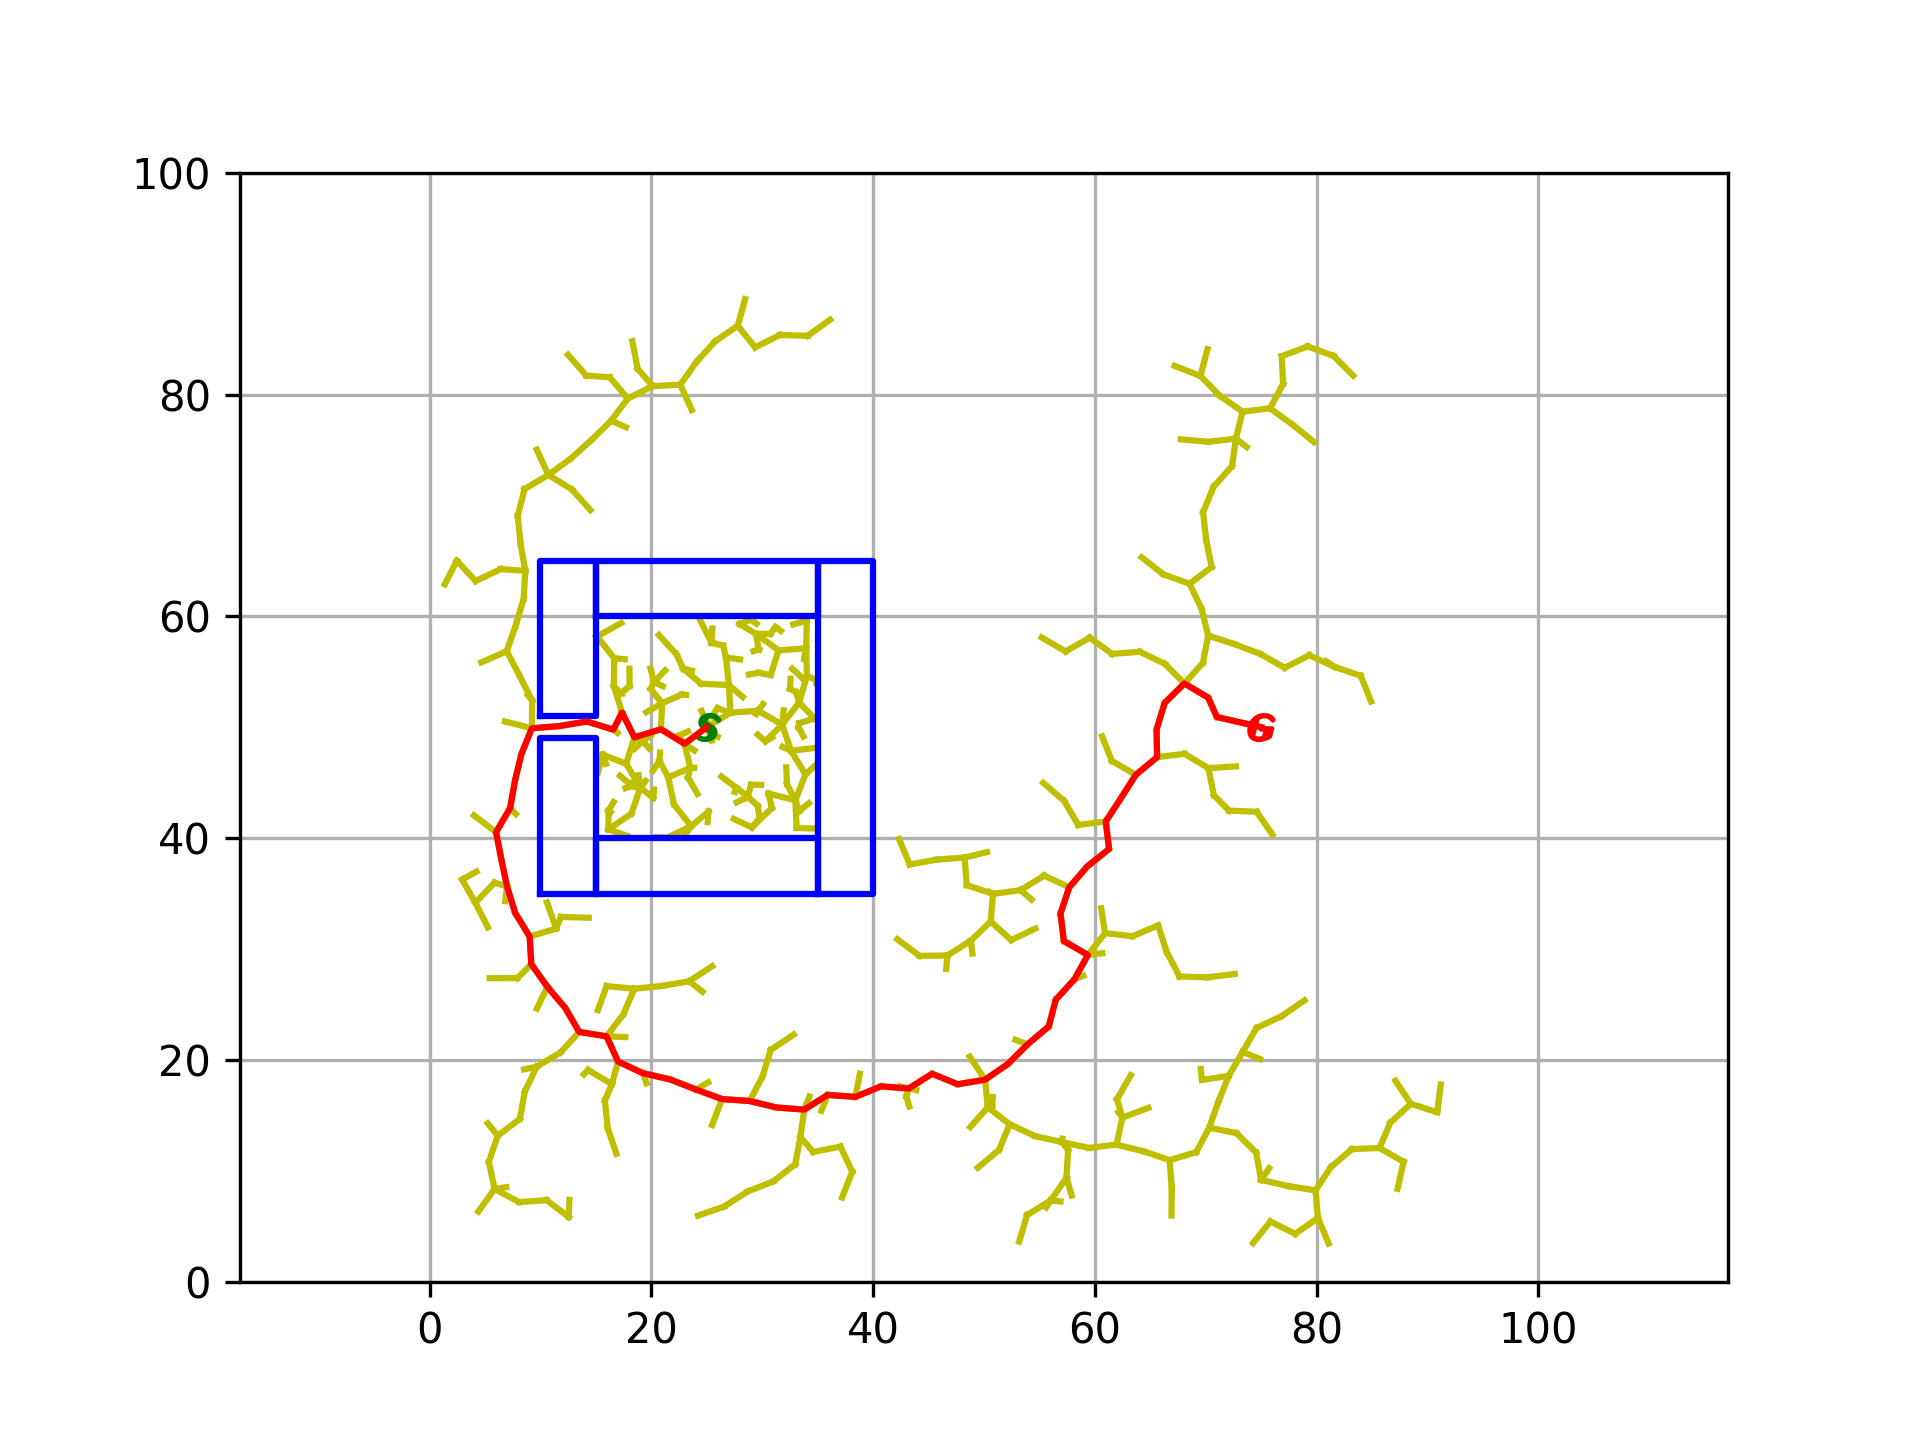
\includegraphics[width=0.45\textwidth]{figures/final_path_RRT_3.png}
    \end{center}
    \caption{Example of RRT on map with bug trap encircling the start}\label{fig:RRT_3}
\end{figure}
\begin{figure}[H]
    \begin{center}
        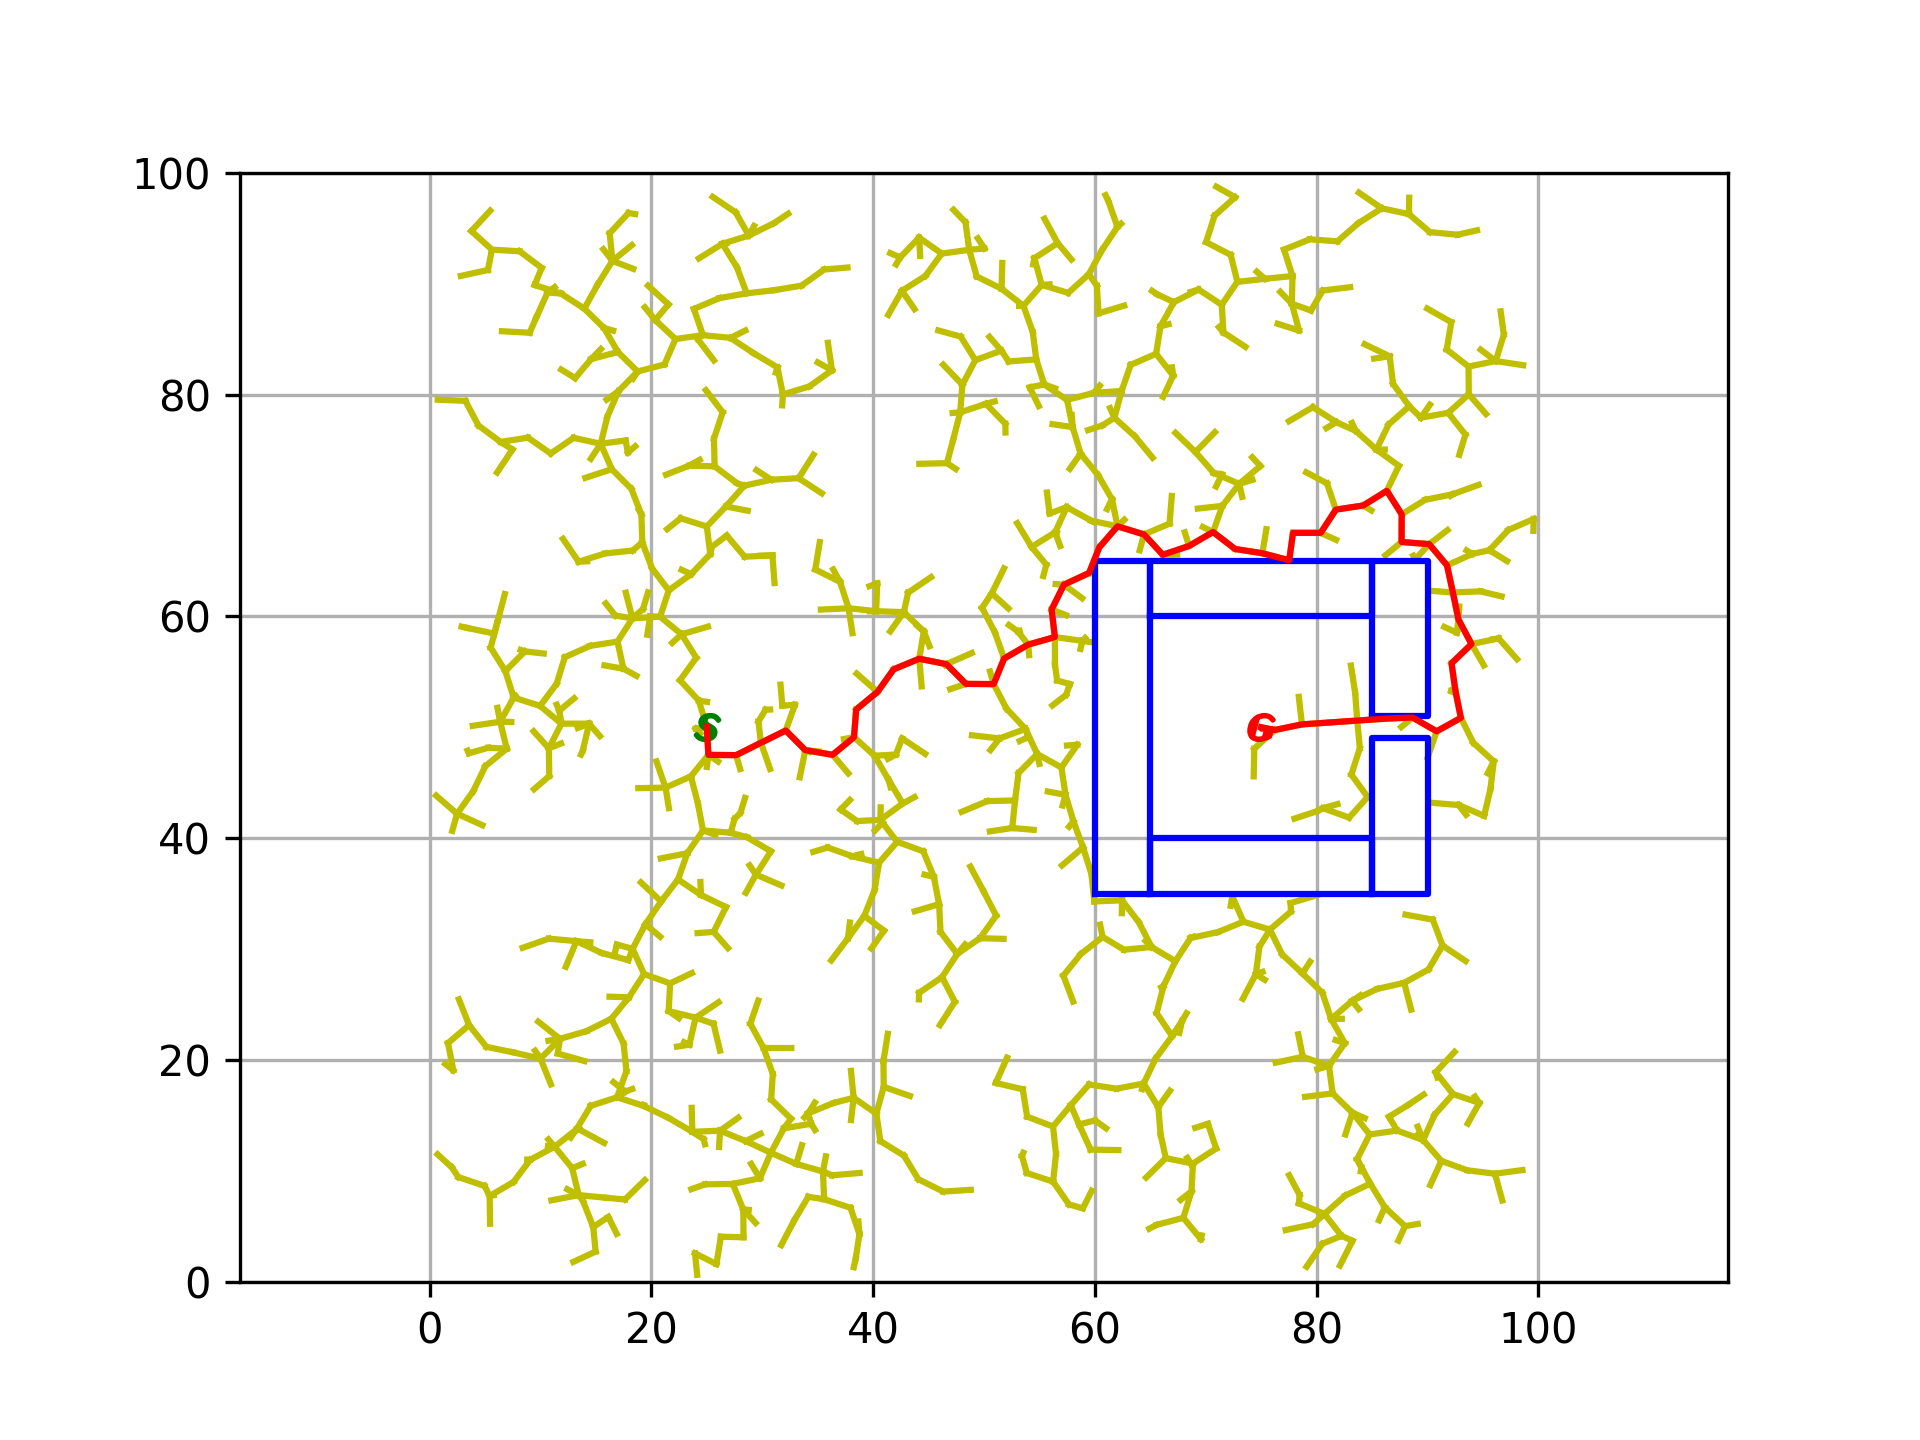
\includegraphics[width=0.45\textwidth]{figures/final_path_RRT_4.png}
    \end{center}
    \caption{Example of RRT on map with bug trap encircling the goal}\label{fig:RRT_4}
\end{figure}
\begin{figure}[H]
    \begin{center}
        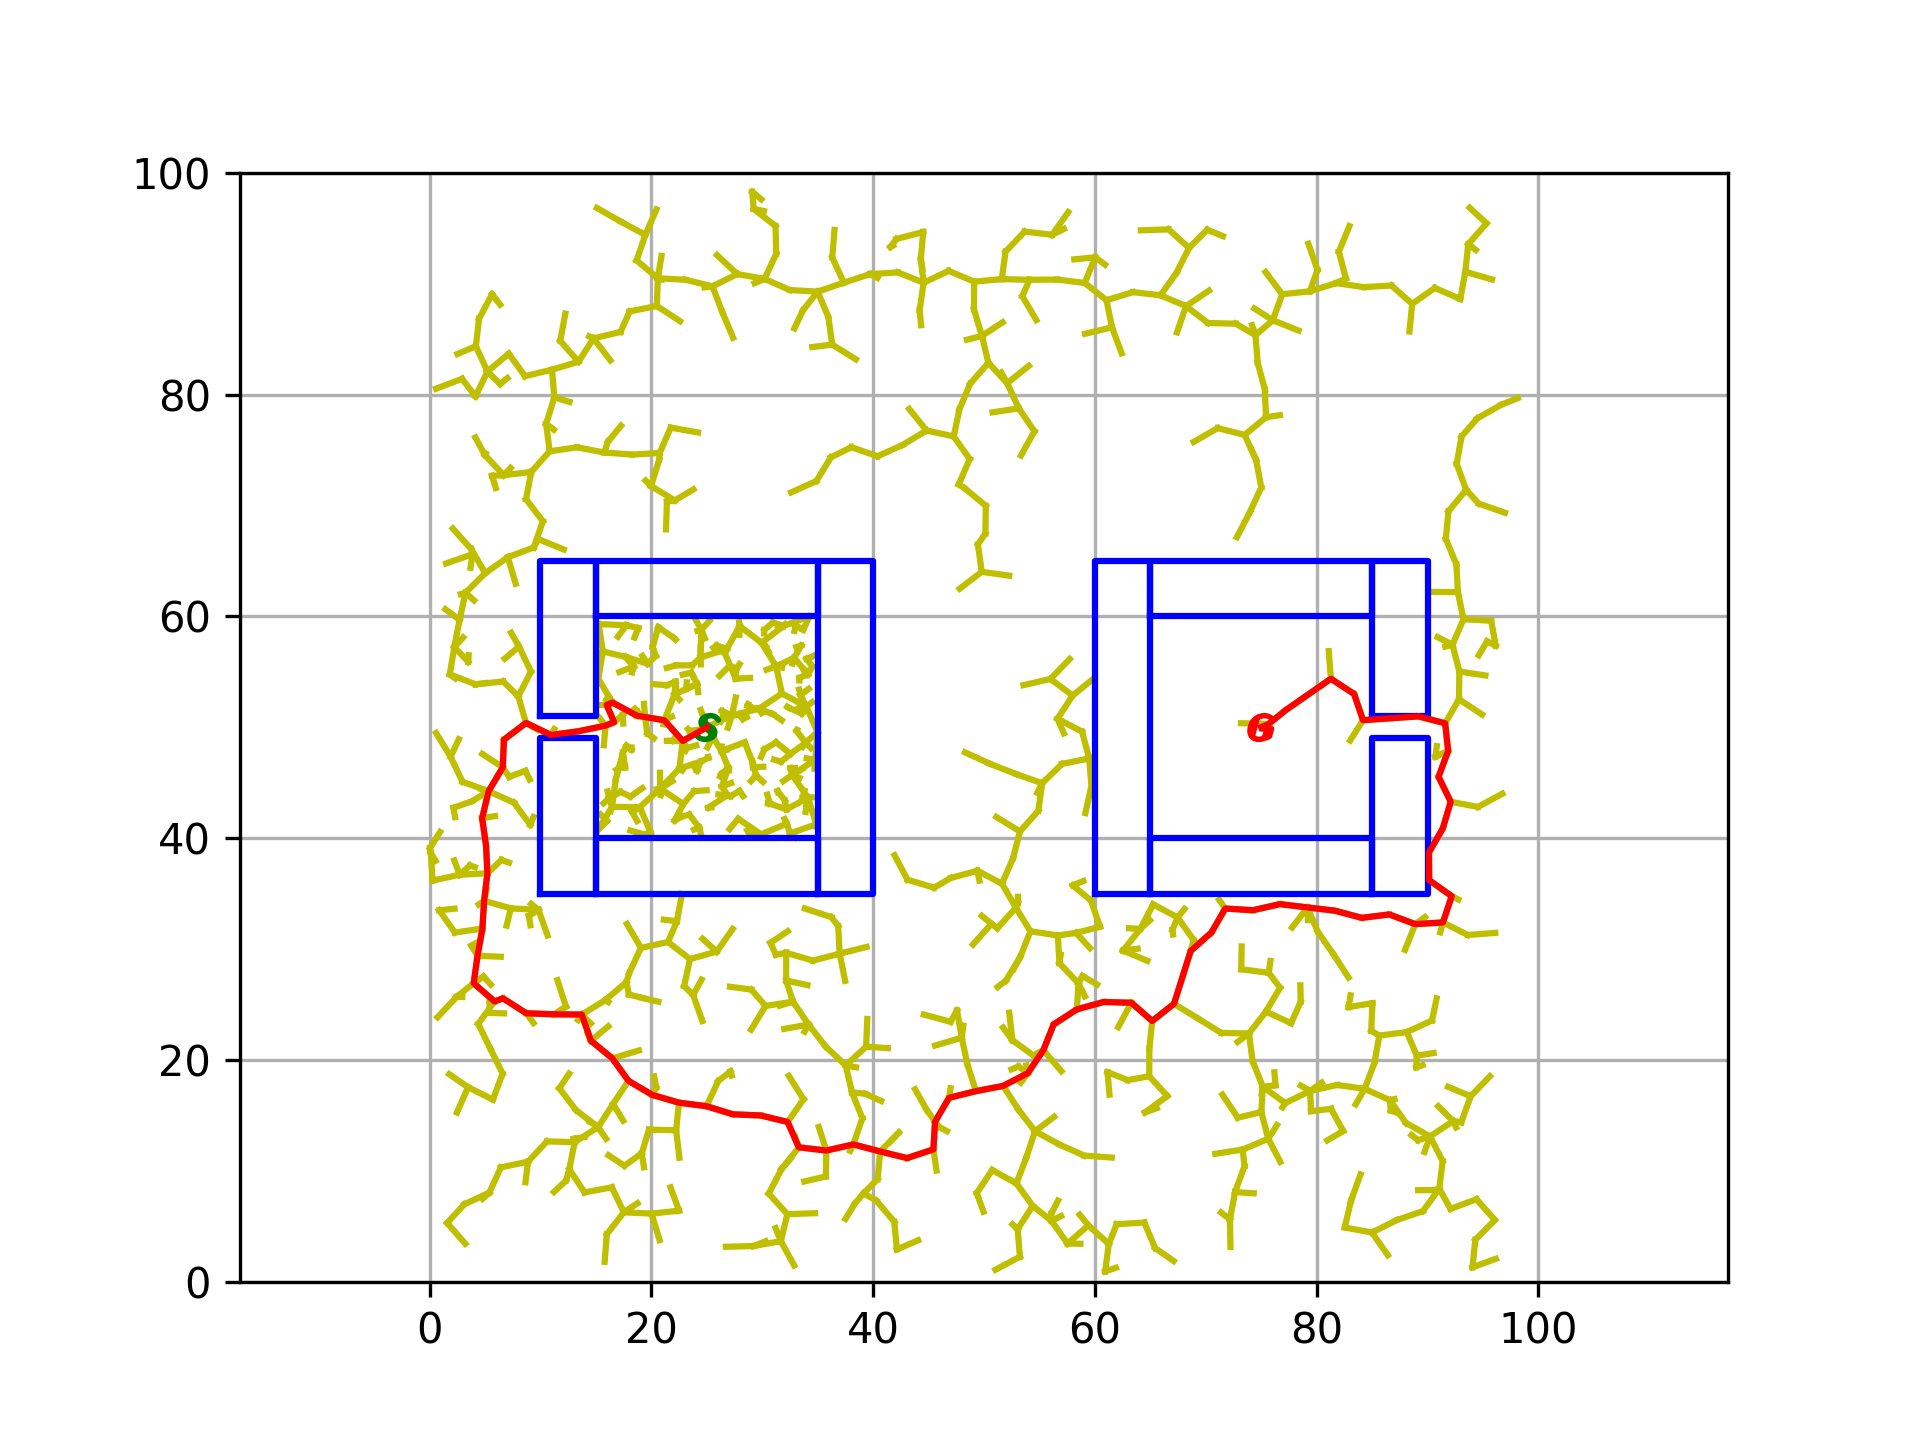
\includegraphics[width=0.45\textwidth]{figures/final_path_RRT_5.png}
    \end{center}
    \caption{Example of RRT on map with bug trap encircling the start and goal}\label{fig:RRT_5}
\end{figure}
\begin{figure}[H]
    \begin{center}
        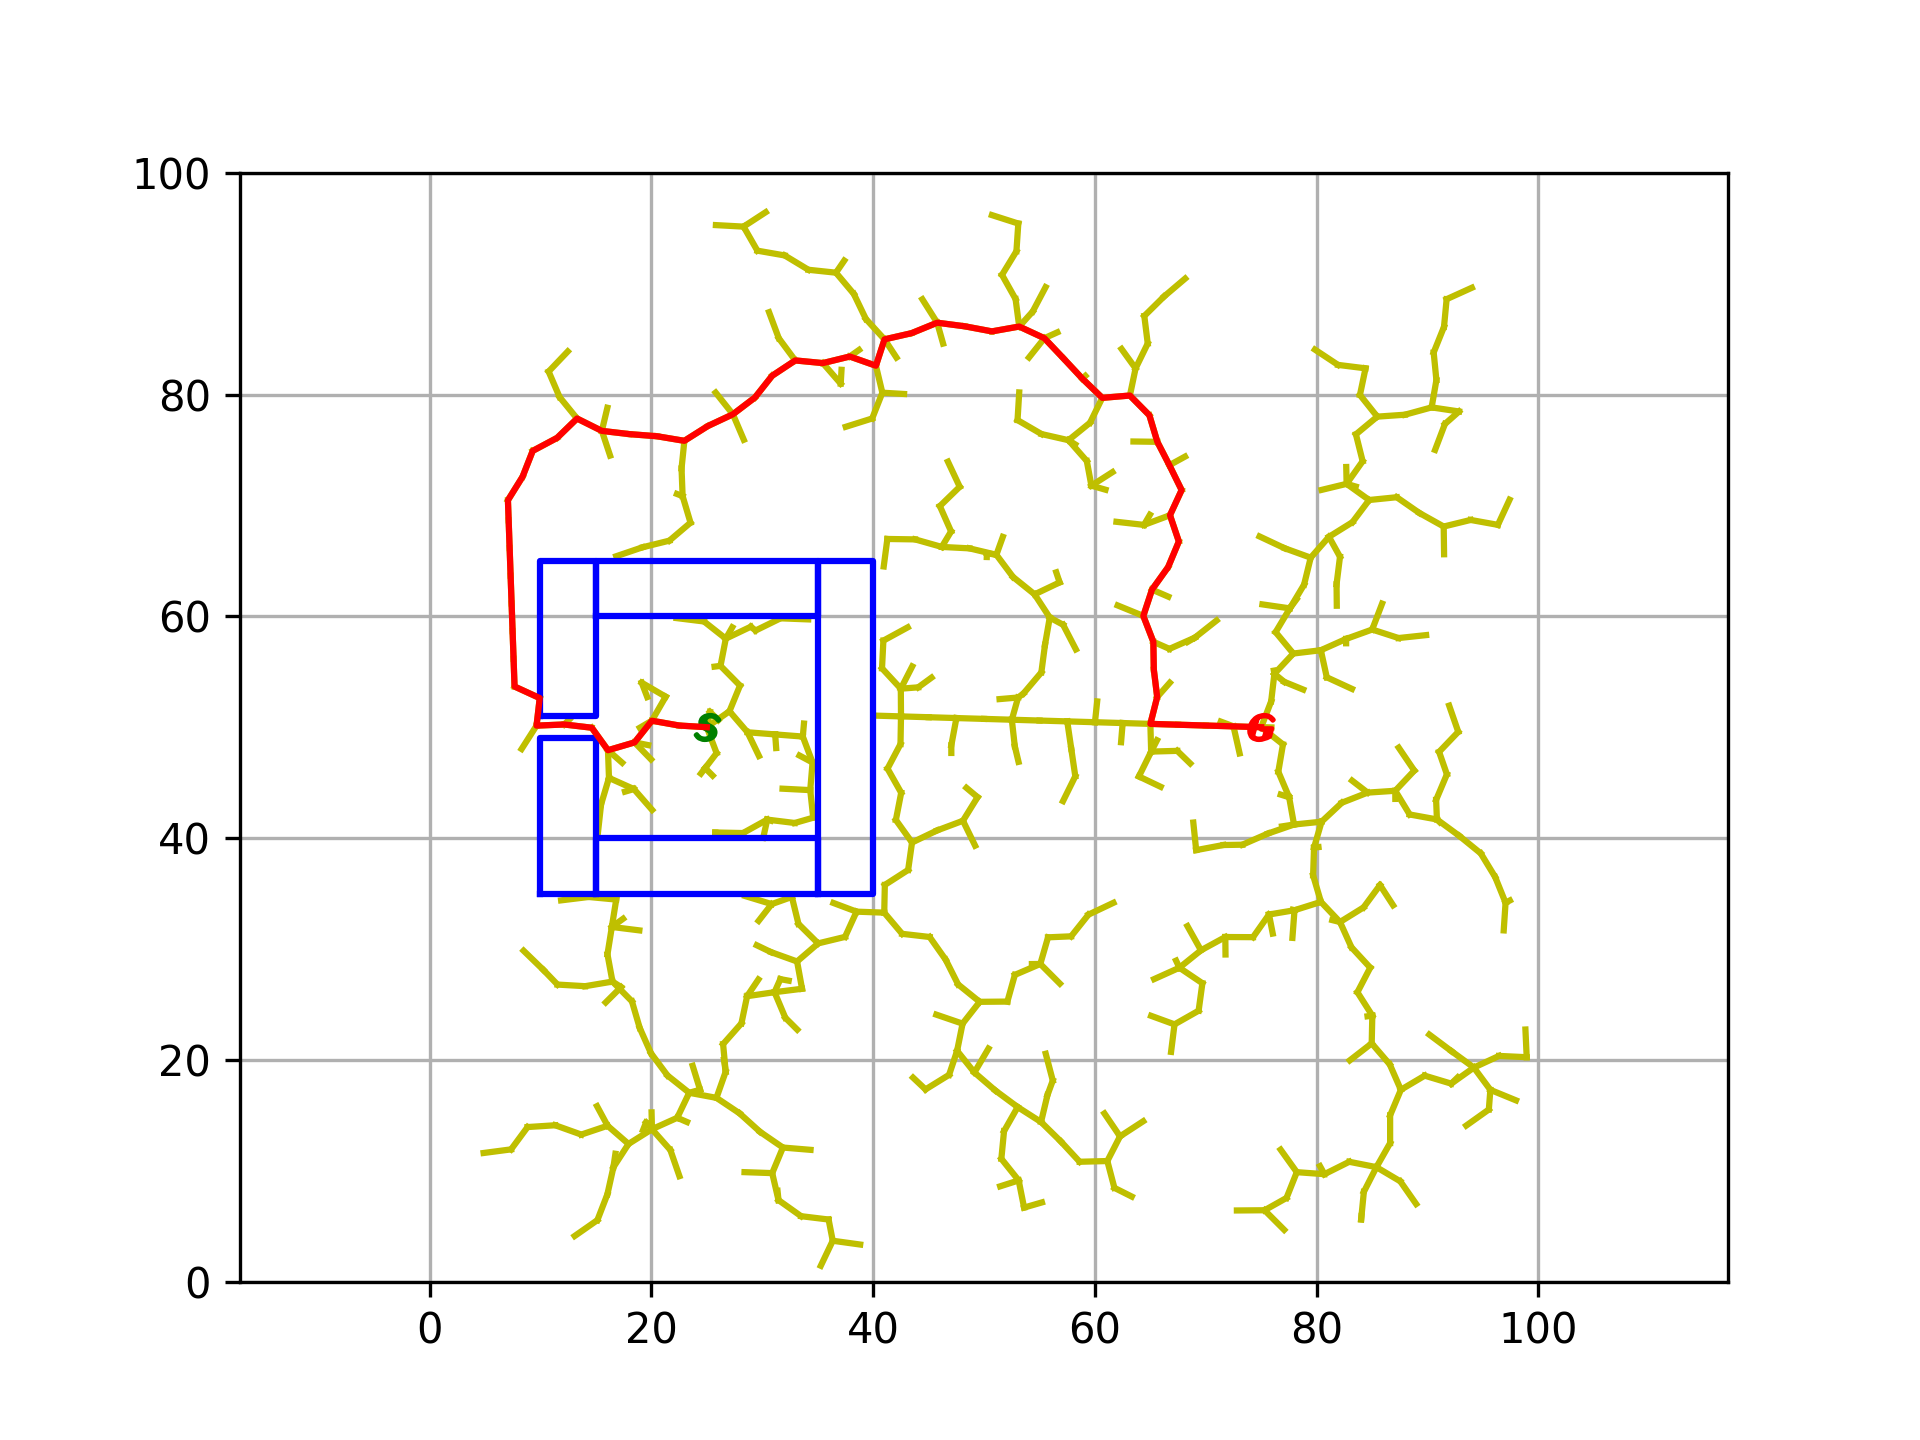
\includegraphics[width=0.45\textwidth]{figures/final_path_RRT_Connect_3.png}
    \end{center}
    \caption{Example of RRT Connect on map with bug trap encircling the start}\label{fig:RRT_Connect_3}
\end{figure}
\begin{figure}[H]
    \begin{center}
        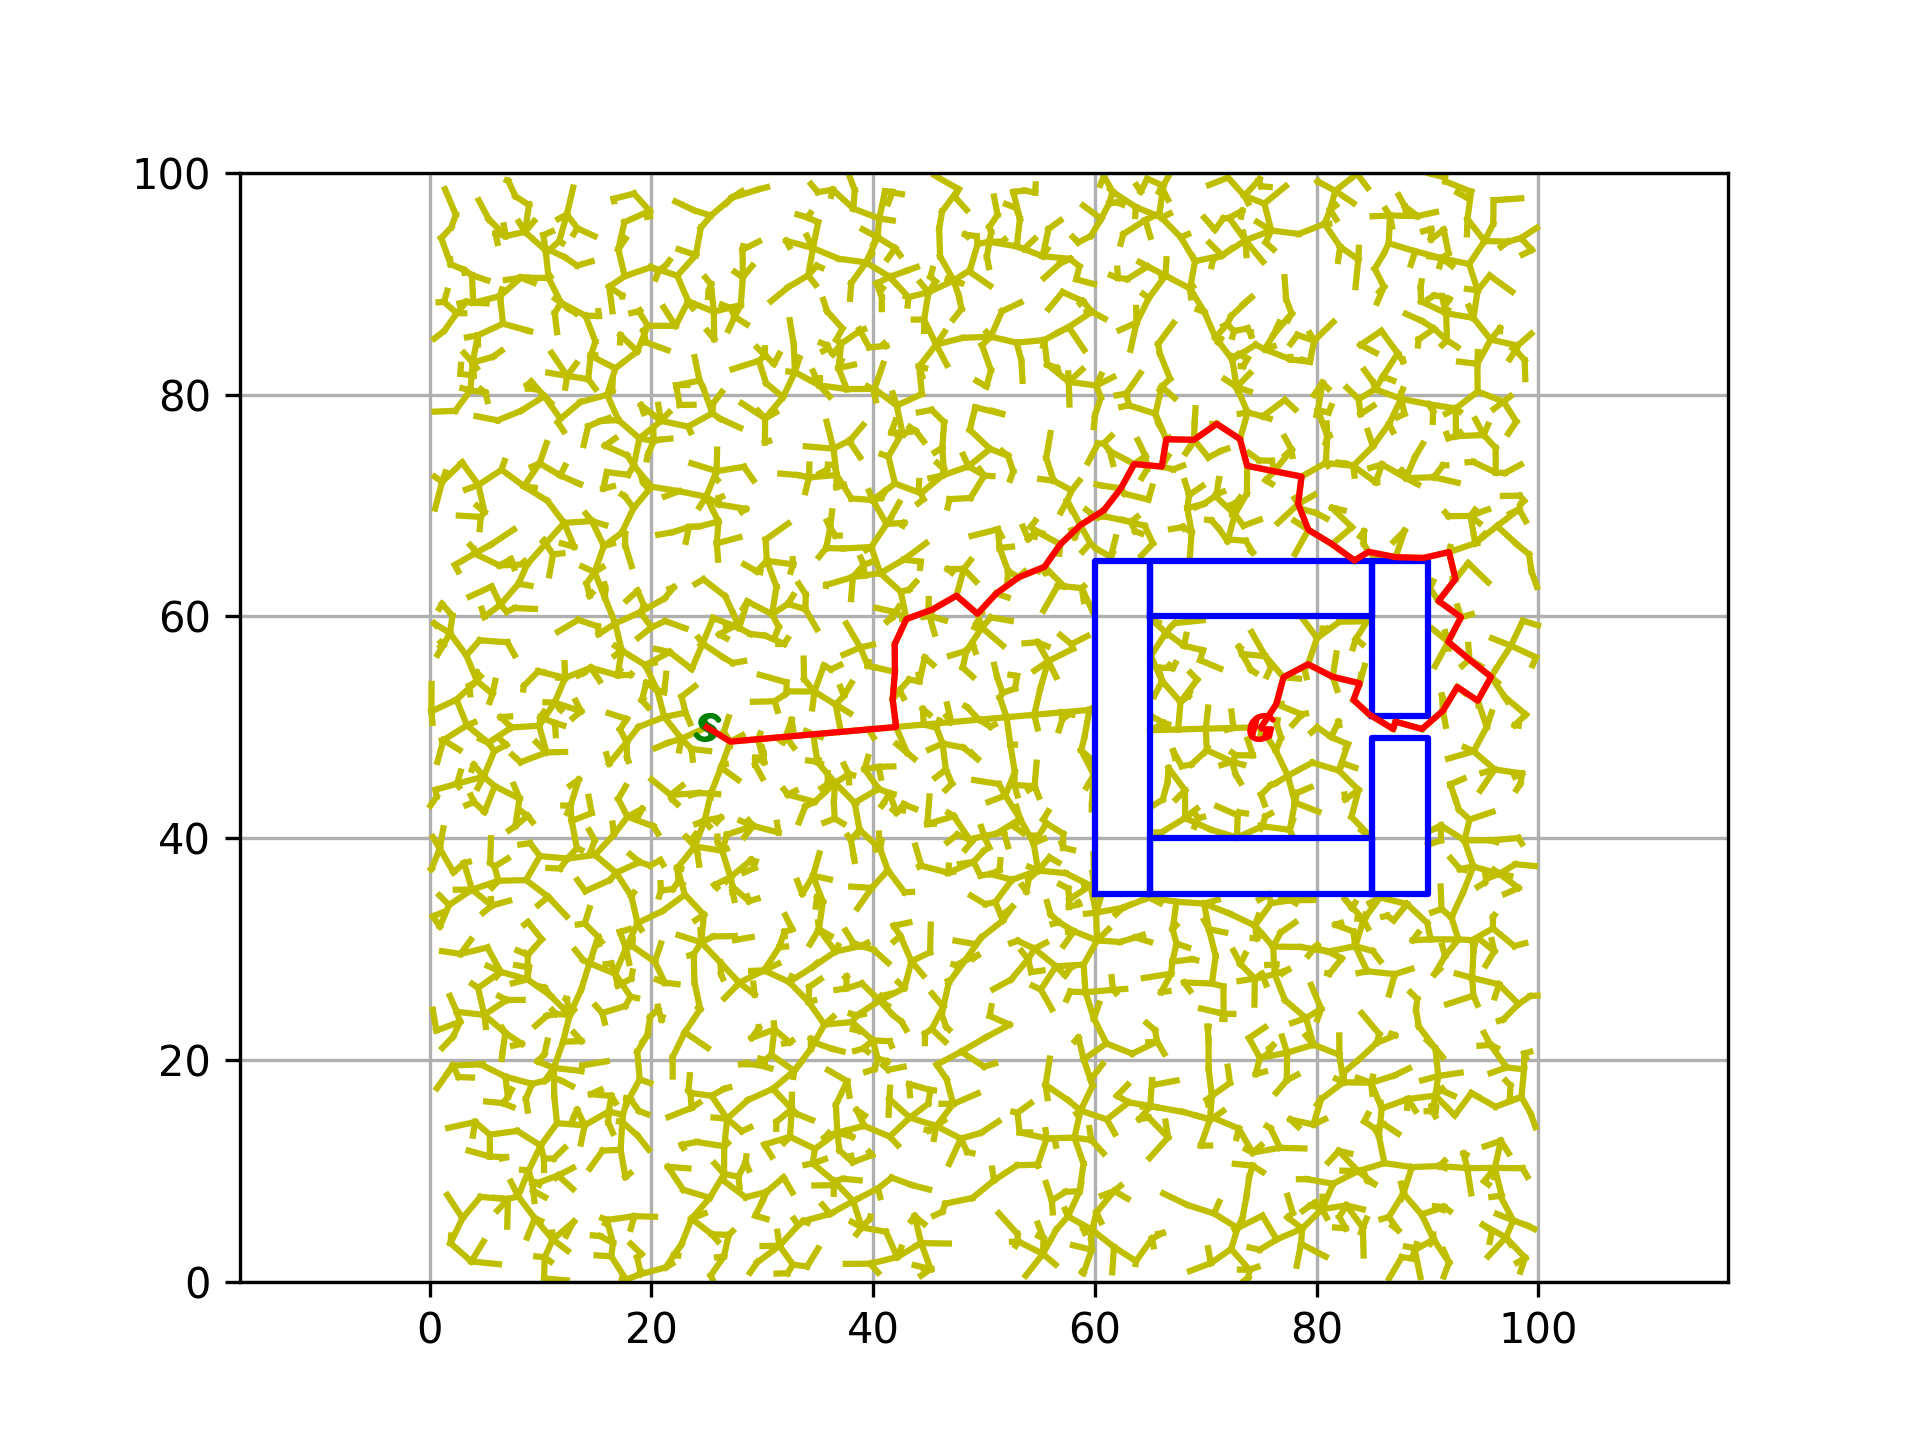
\includegraphics[width=0.45\textwidth]{figures/final_path_RRT_Connect_4.png}
    \end{center}
    \caption{Example of RRT Connect on map with bug trap encircling the goal}\label{fig:RRT_Connect_4}
\end{figure}
\begin{figure}[H]
    \begin{center}
        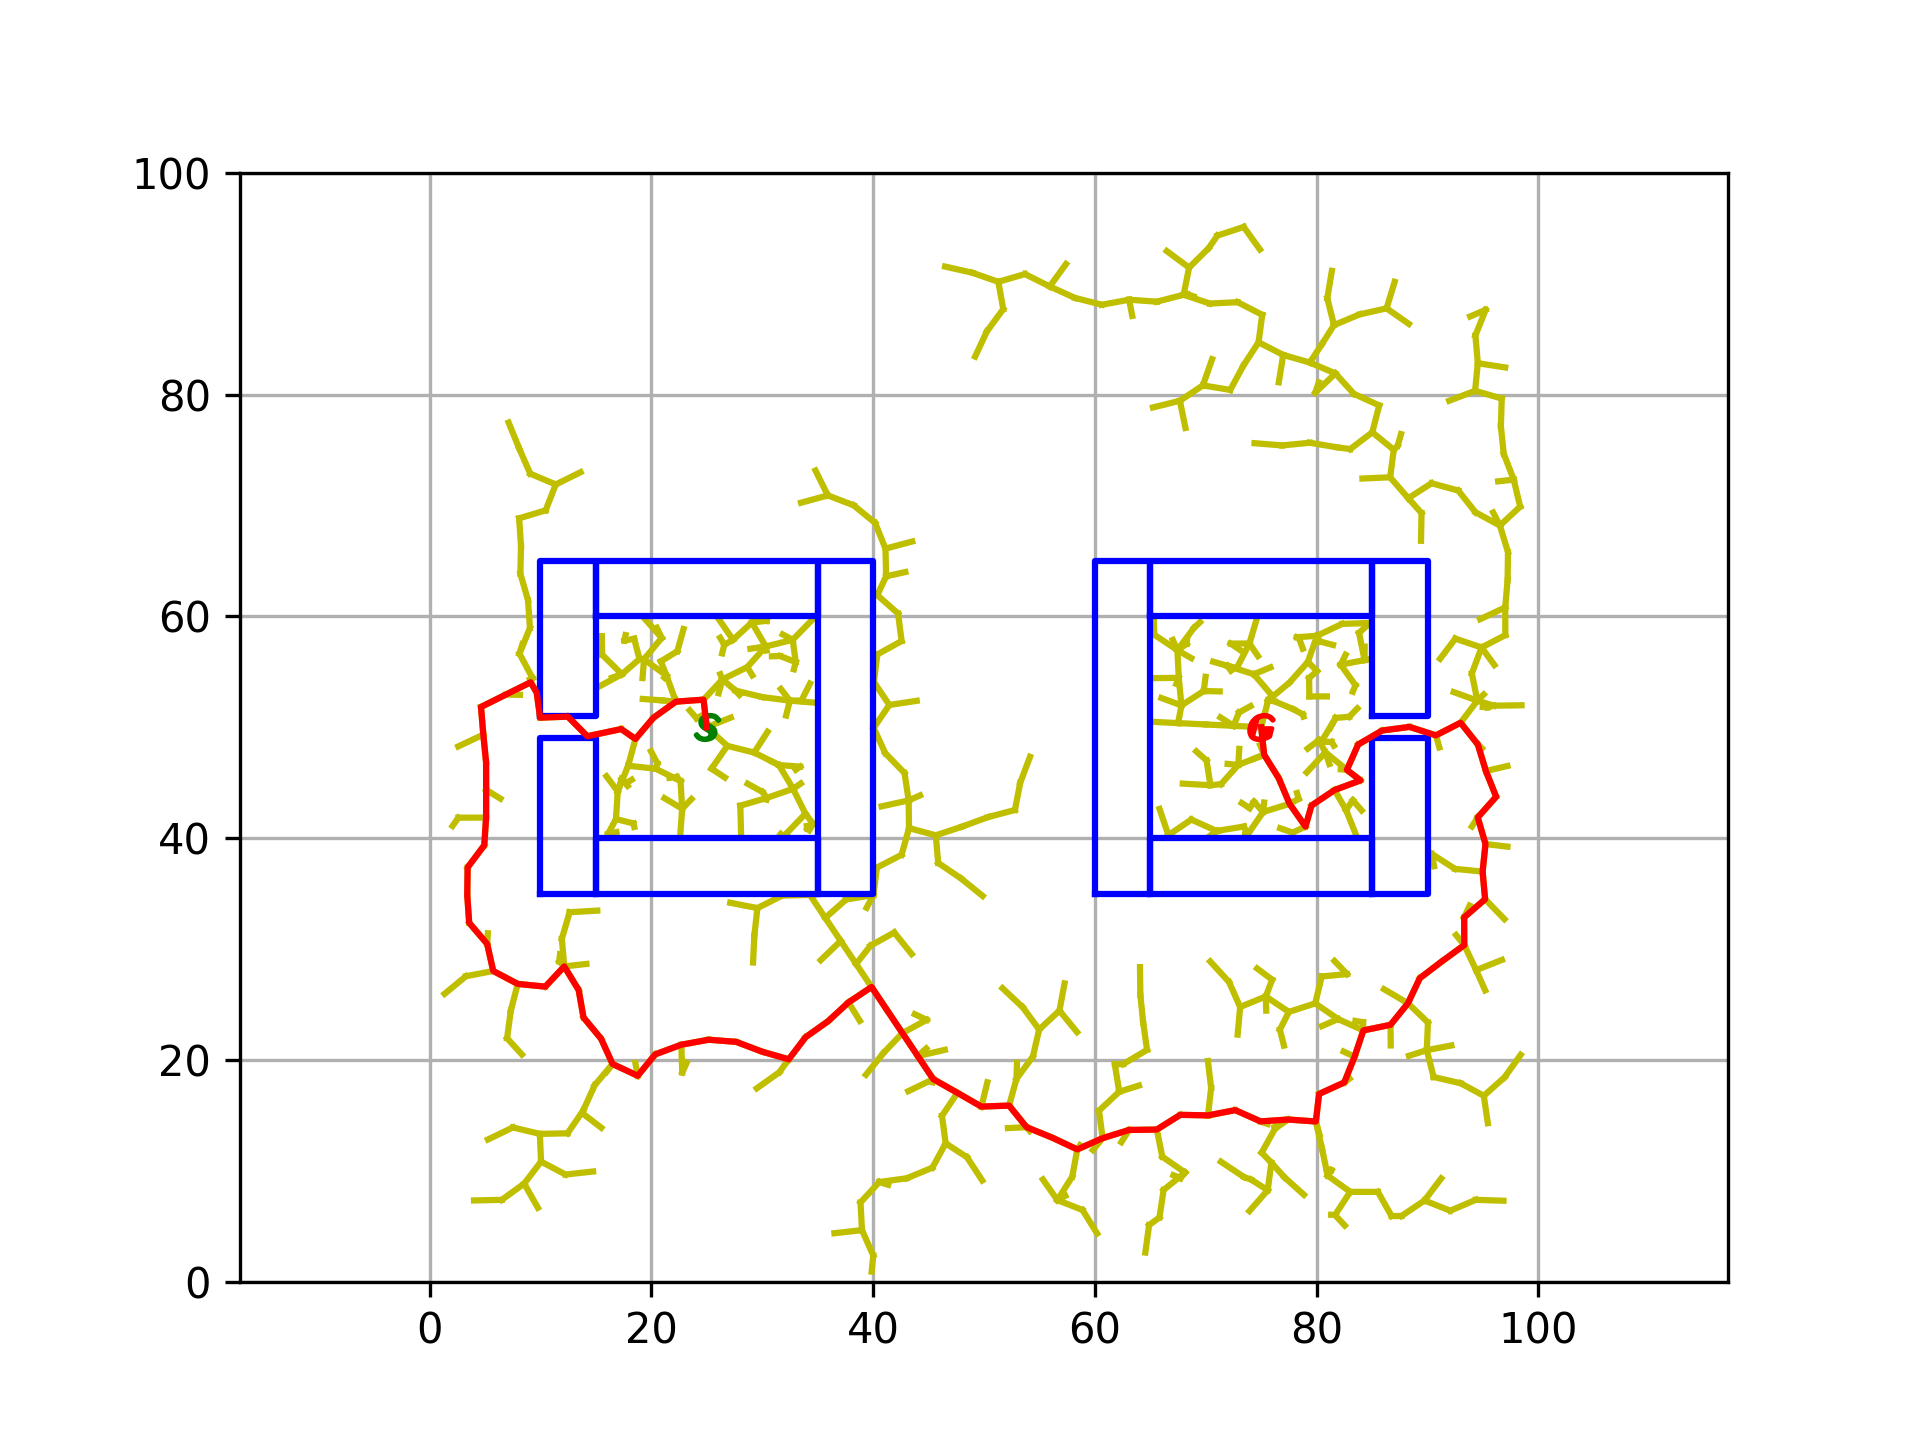
\includegraphics[width=0.45\textwidth]{figures/final_path_RRT_Connect_5.png}
    \end{center}
    \caption{Example of RRT Connect on map with bug trap encircling the start and goal}\label{fig:RRT_Connect_5}
\end{figure}
and histograms
\begin{figure}[H]
    \begin{center}
        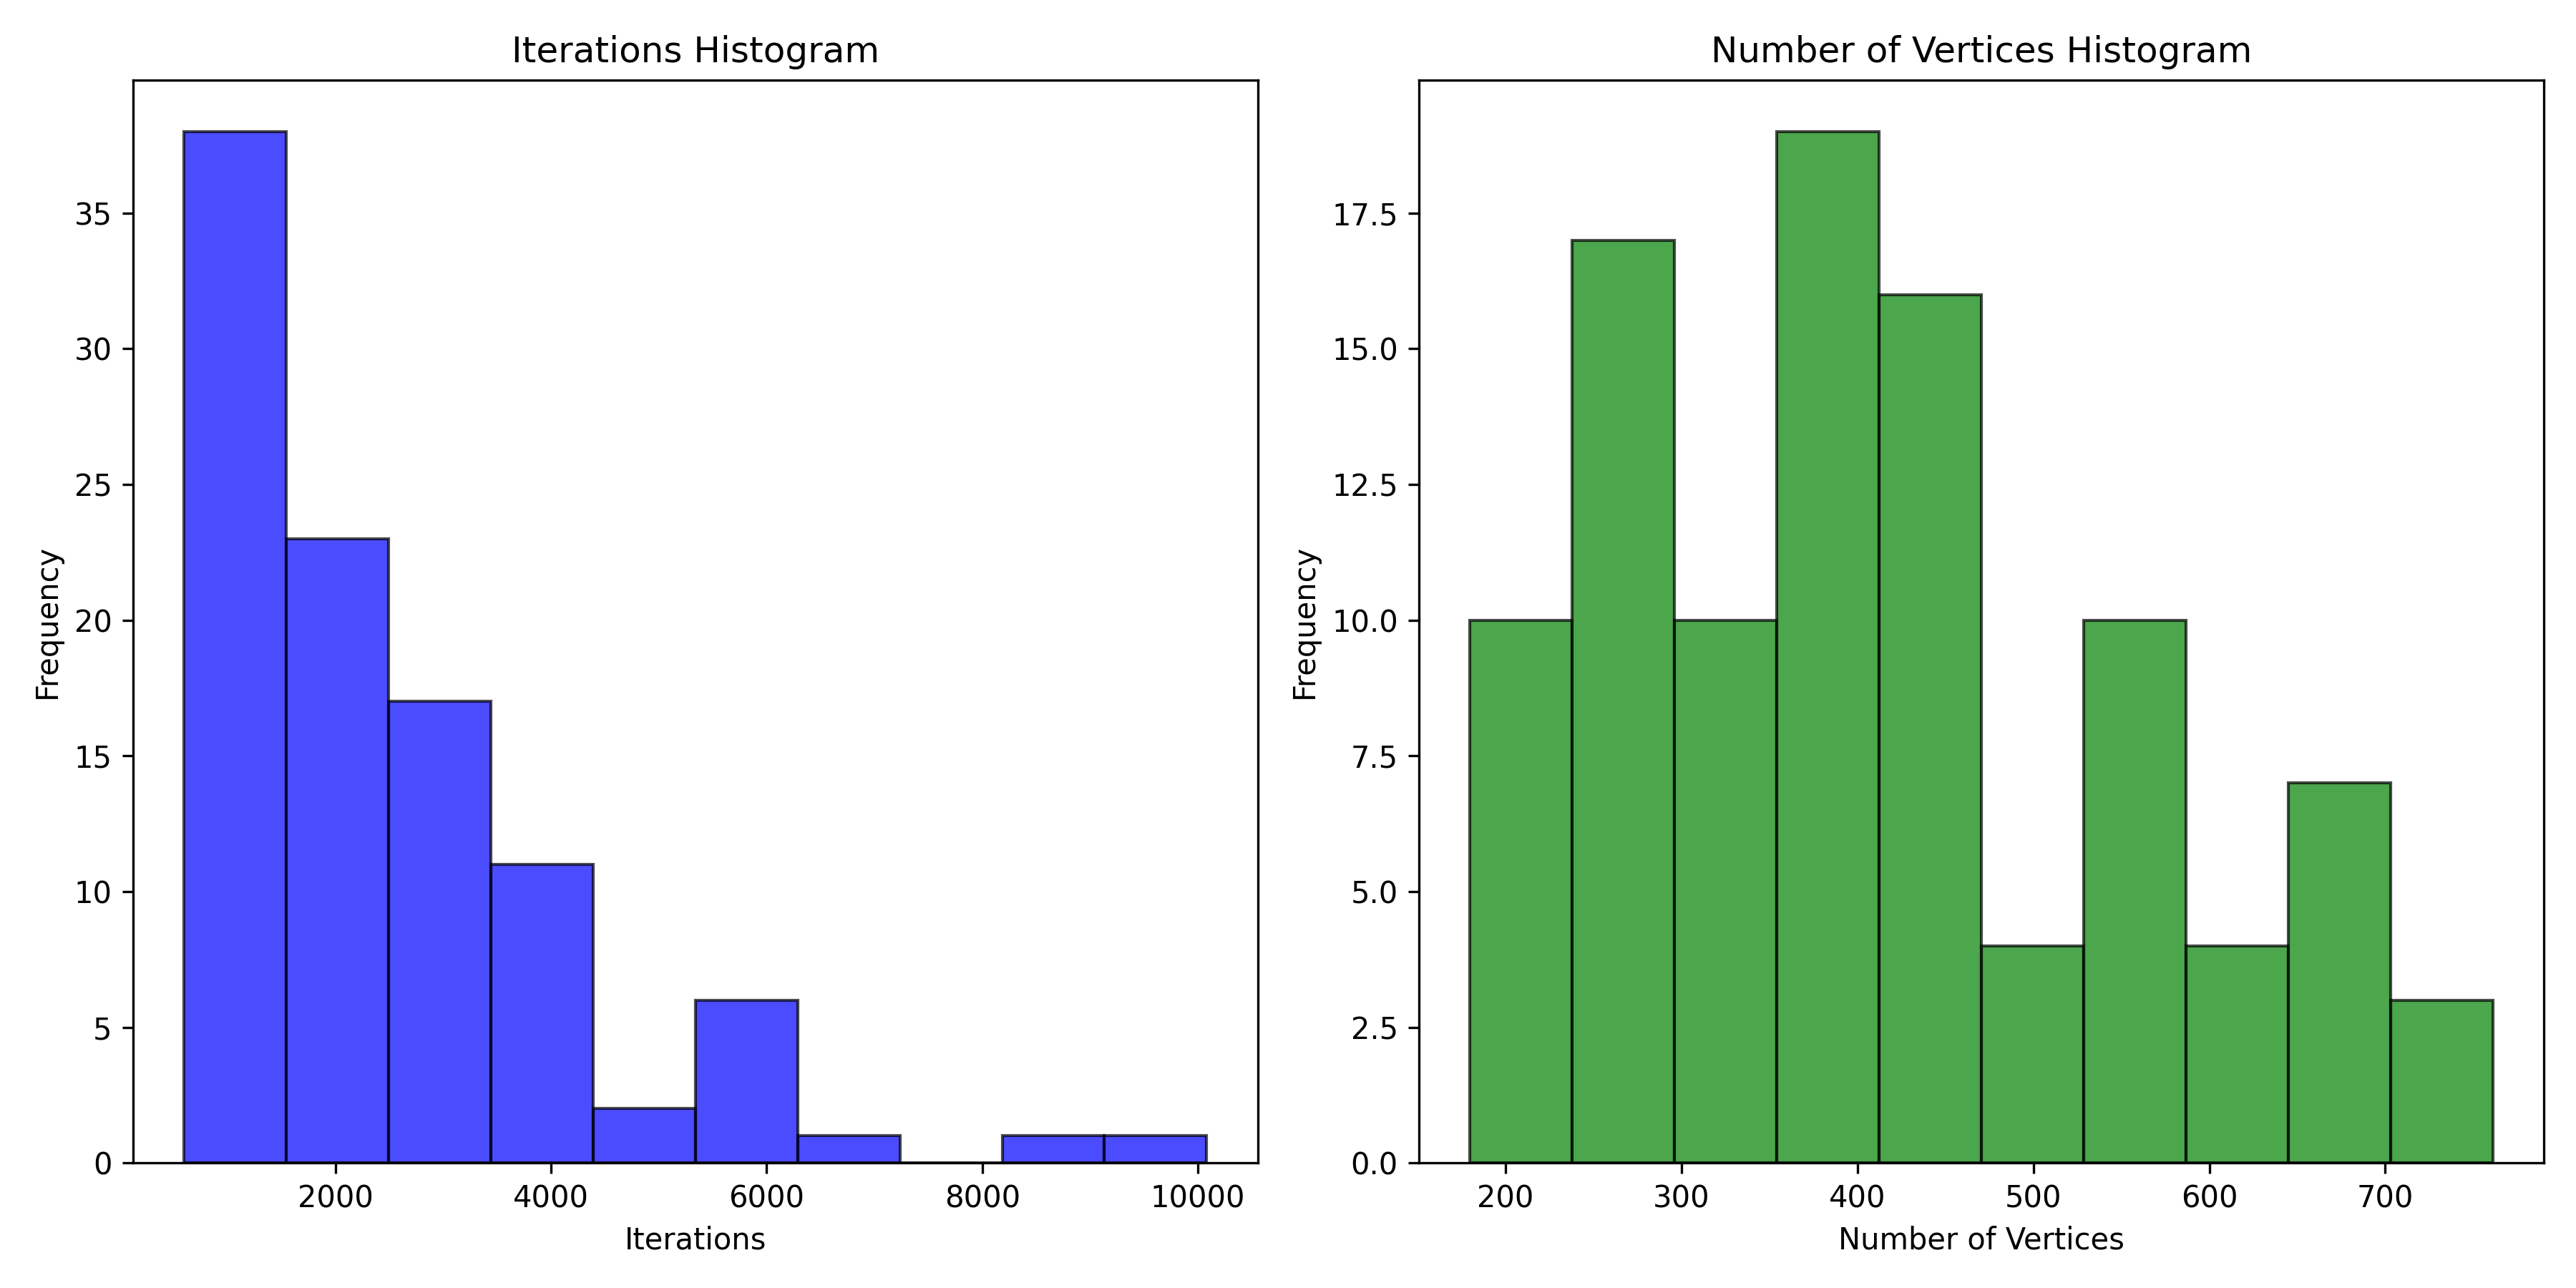
\includegraphics[width=0.65\textwidth]{figures/hist_RRT_3.png}
    \end{center}
    \caption{Histogram depicting number of iterations and number of
    vertices of RRT with bug trap encircling start over 100
trials}\label{fig:hist_RRT_3}
\end{figure}
\begin{figure}[H]
    \begin{center}
        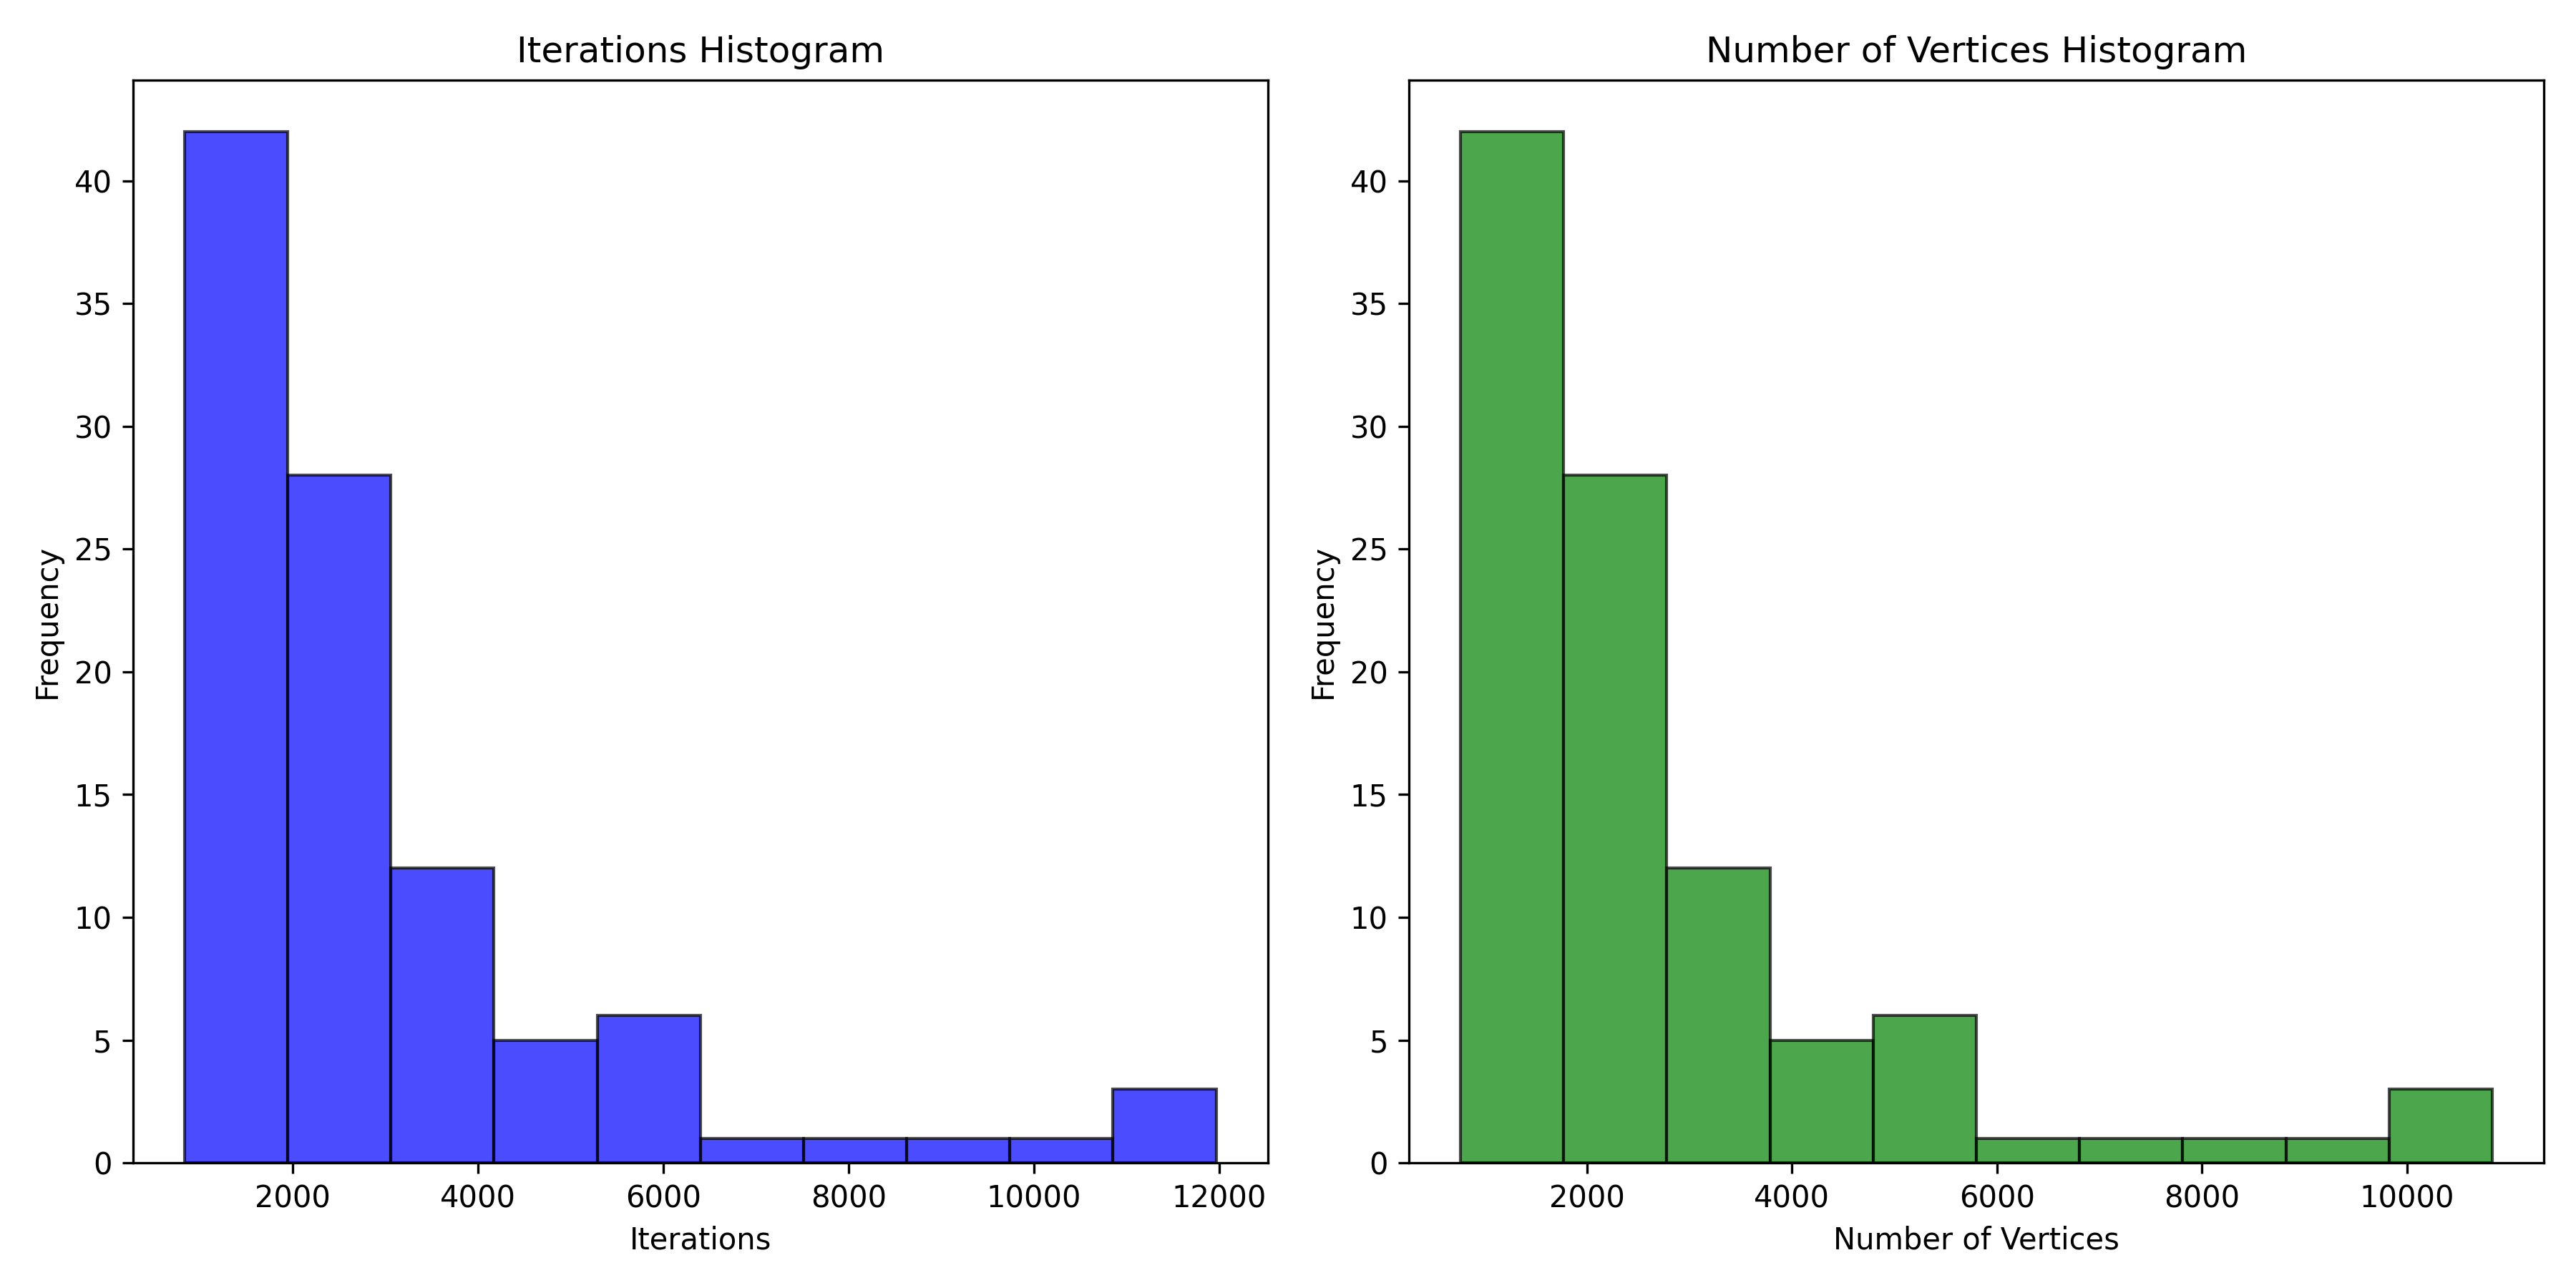
\includegraphics[width=0.65\textwidth]{figures/hist_RRT_4.png}
    \end{center}
    \caption{Histogram depicting number of iterations and number of
    vertices of RRT with bug trap encircling goal over 100
trials}\label{fig:hist_RRT_4}
\end{figure}
\begin{figure}[H]
    \begin{center}
        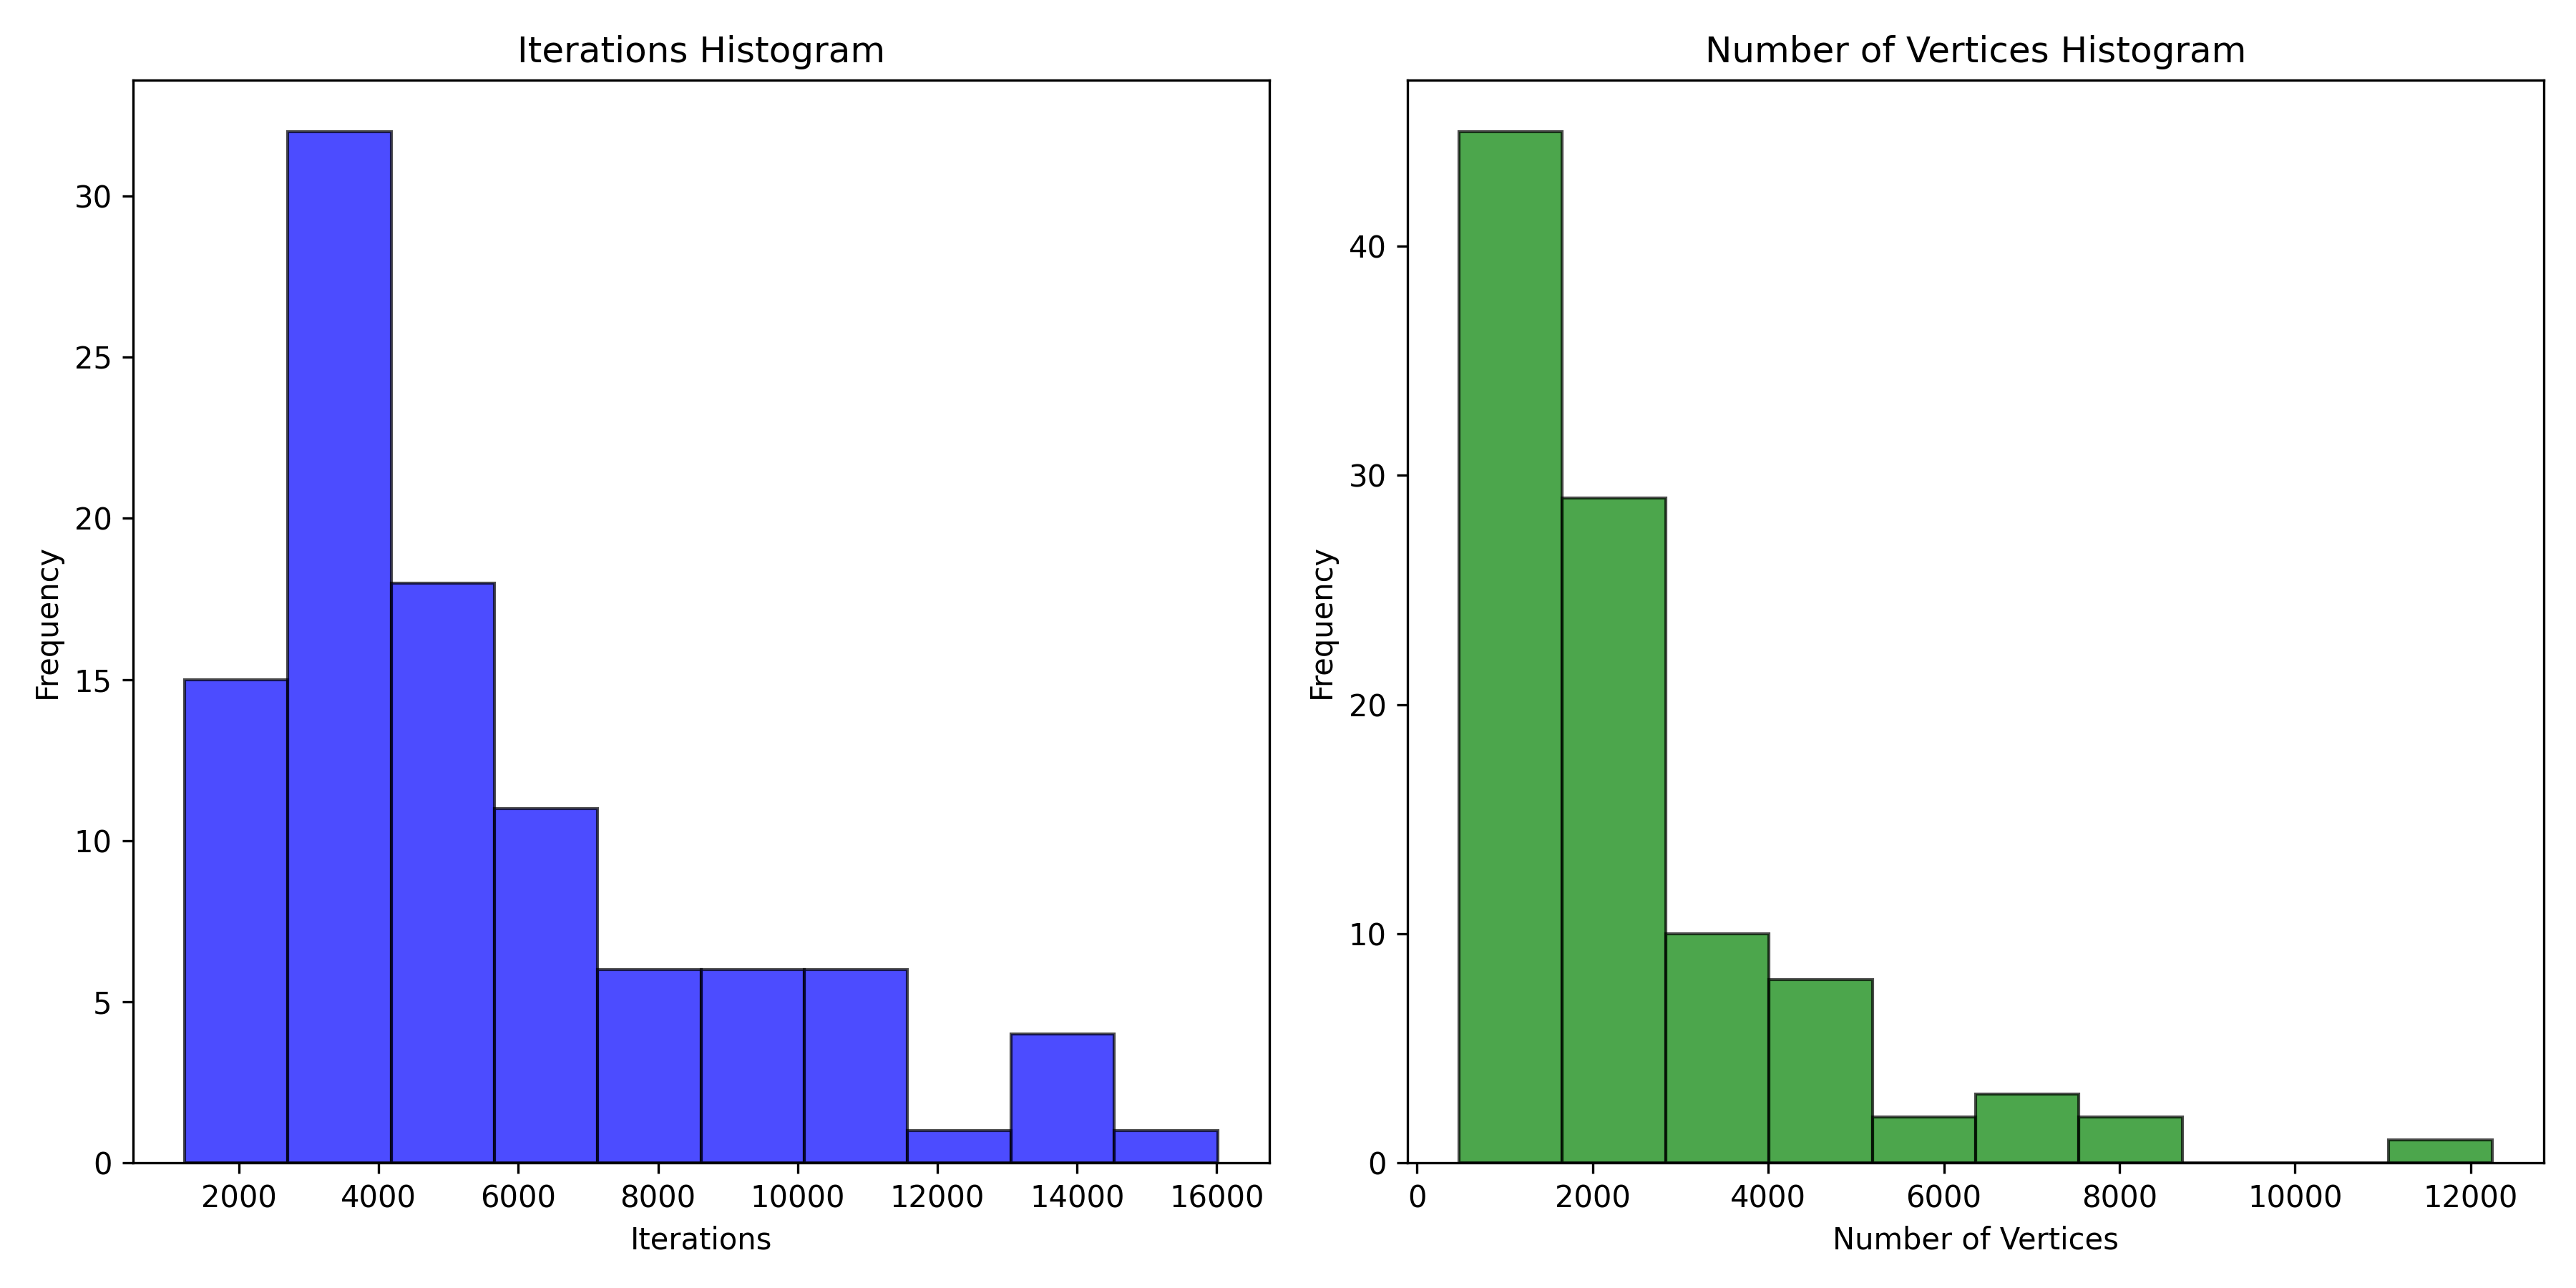
\includegraphics[width=0.65\textwidth]{figures/hist_RRT_5.png}
    \end{center}
    \caption{Histogram depicting number of iterations and number of
    vertices of RRT with bug trap encircling start and goal over 100
trials}\label{fig:hist_RRT_5}
\end{figure}
\begin{figure}[H]
    \begin{center}
        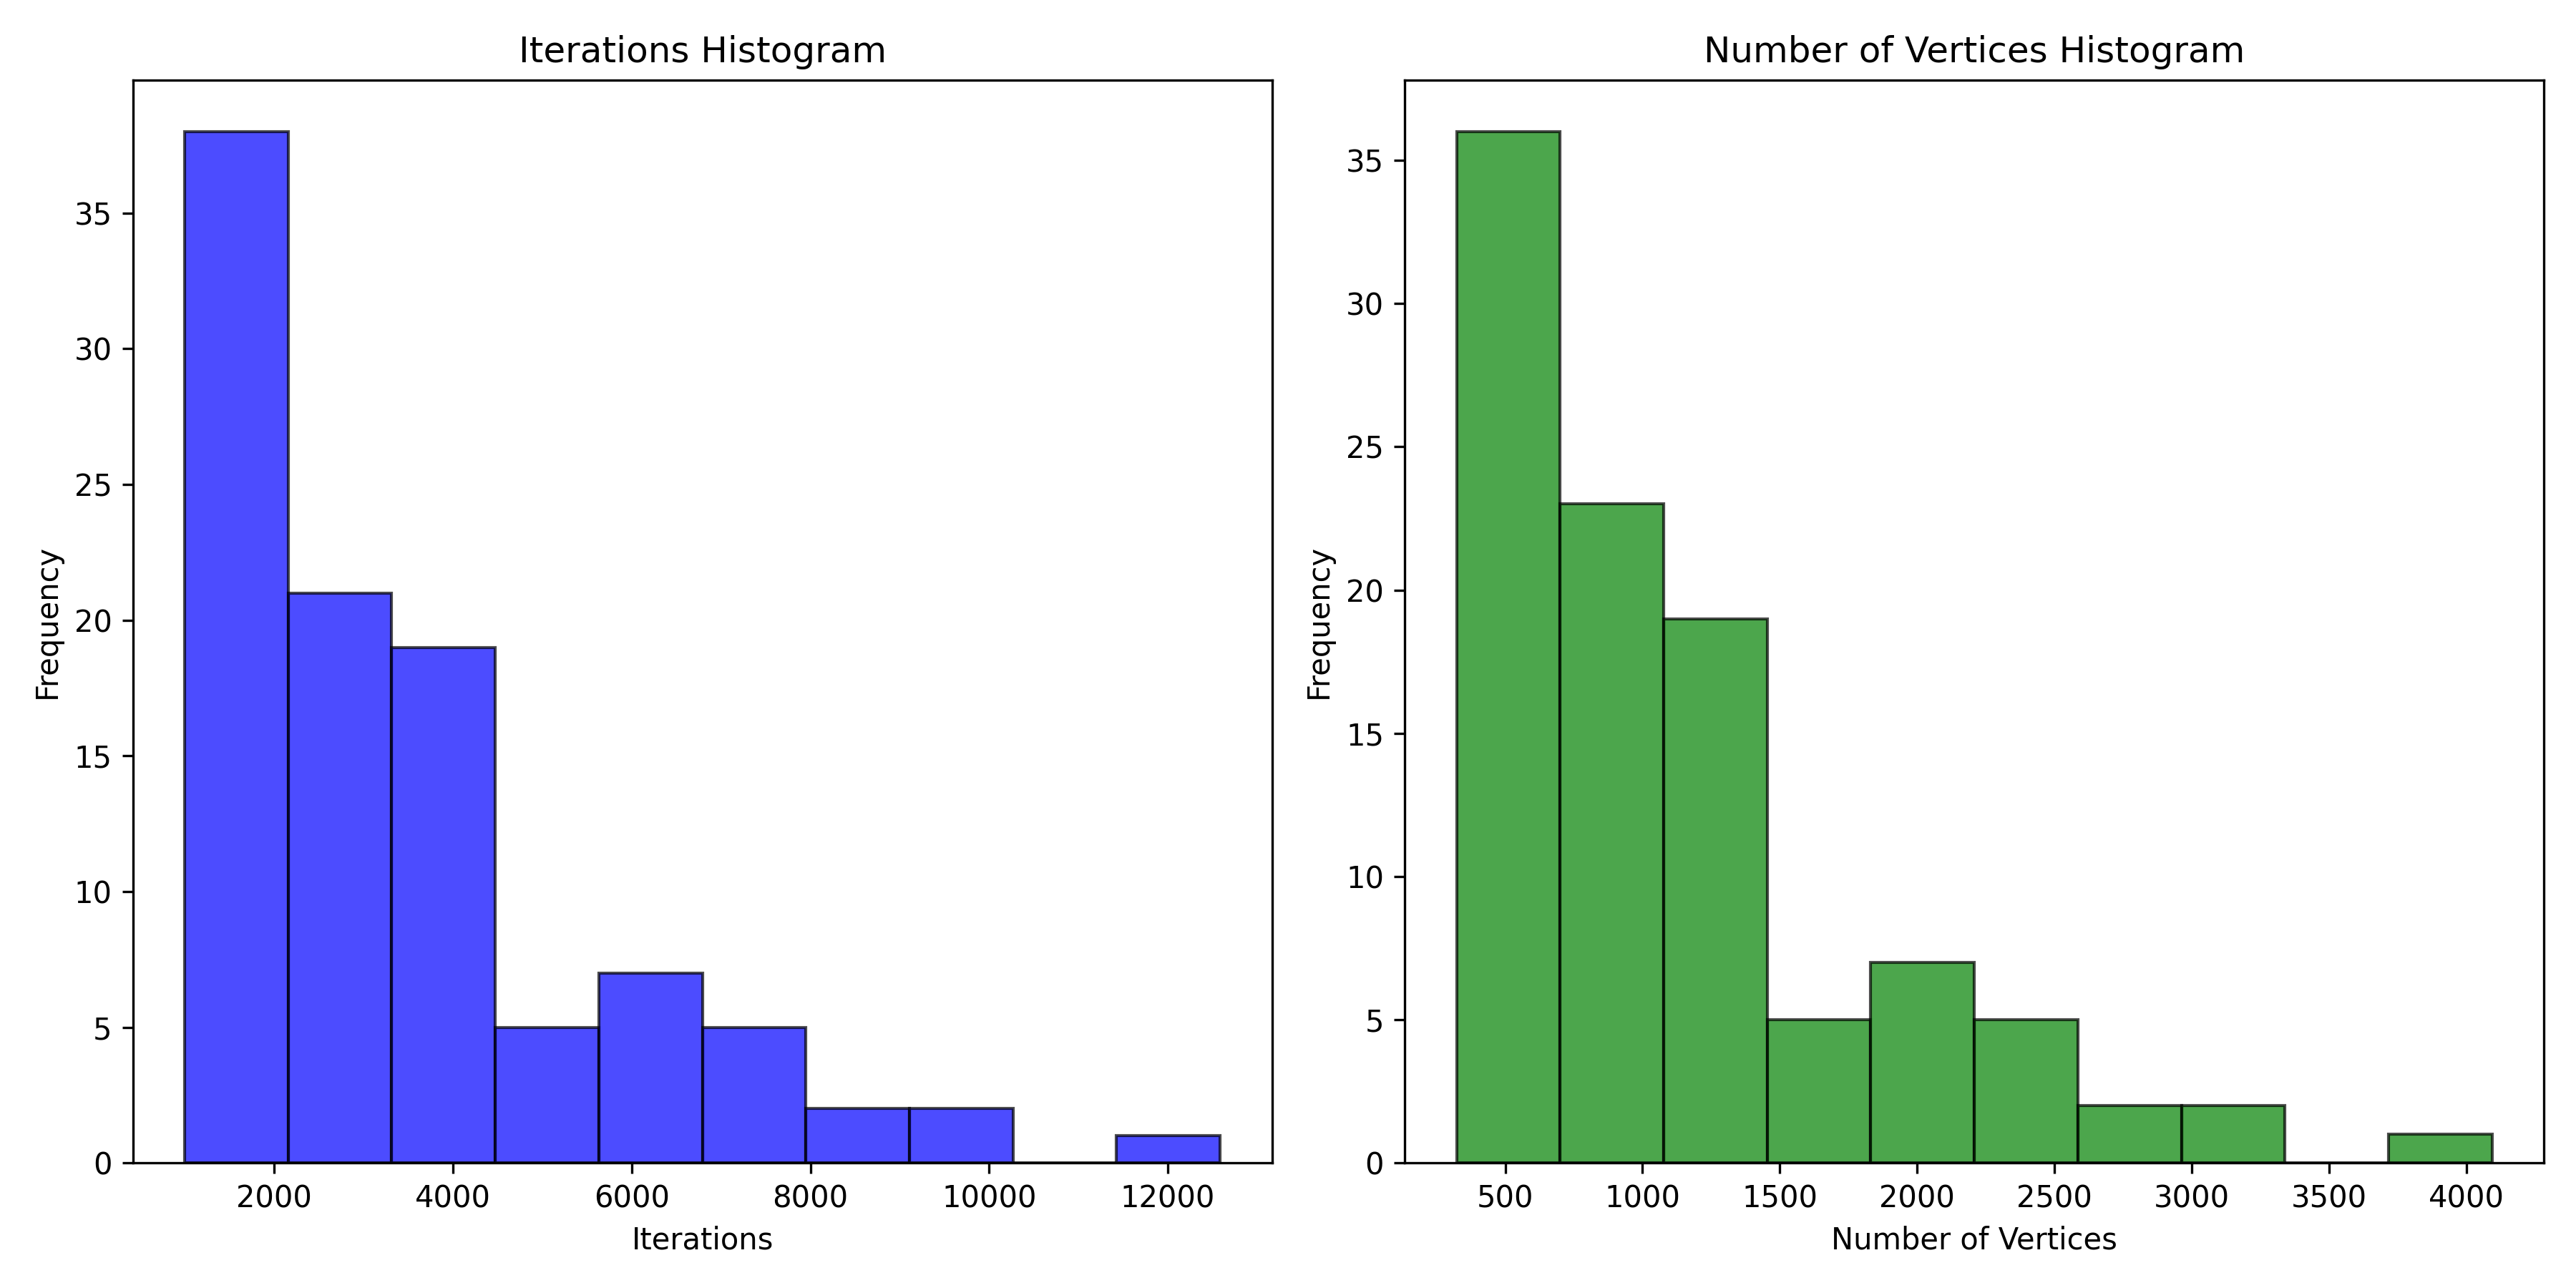
\includegraphics[width=0.65\textwidth]{figures/hist_RRT_Connect_3.png}
    \end{center}
    \caption{Histogram depicting number of iterations and number of
    vertices of RRT Connect with bug trap encircling start over 100
trials}\label{fig:hist_RRT_Connect_3}
\end{figure}
\begin{figure}[H]
    \begin{center}
        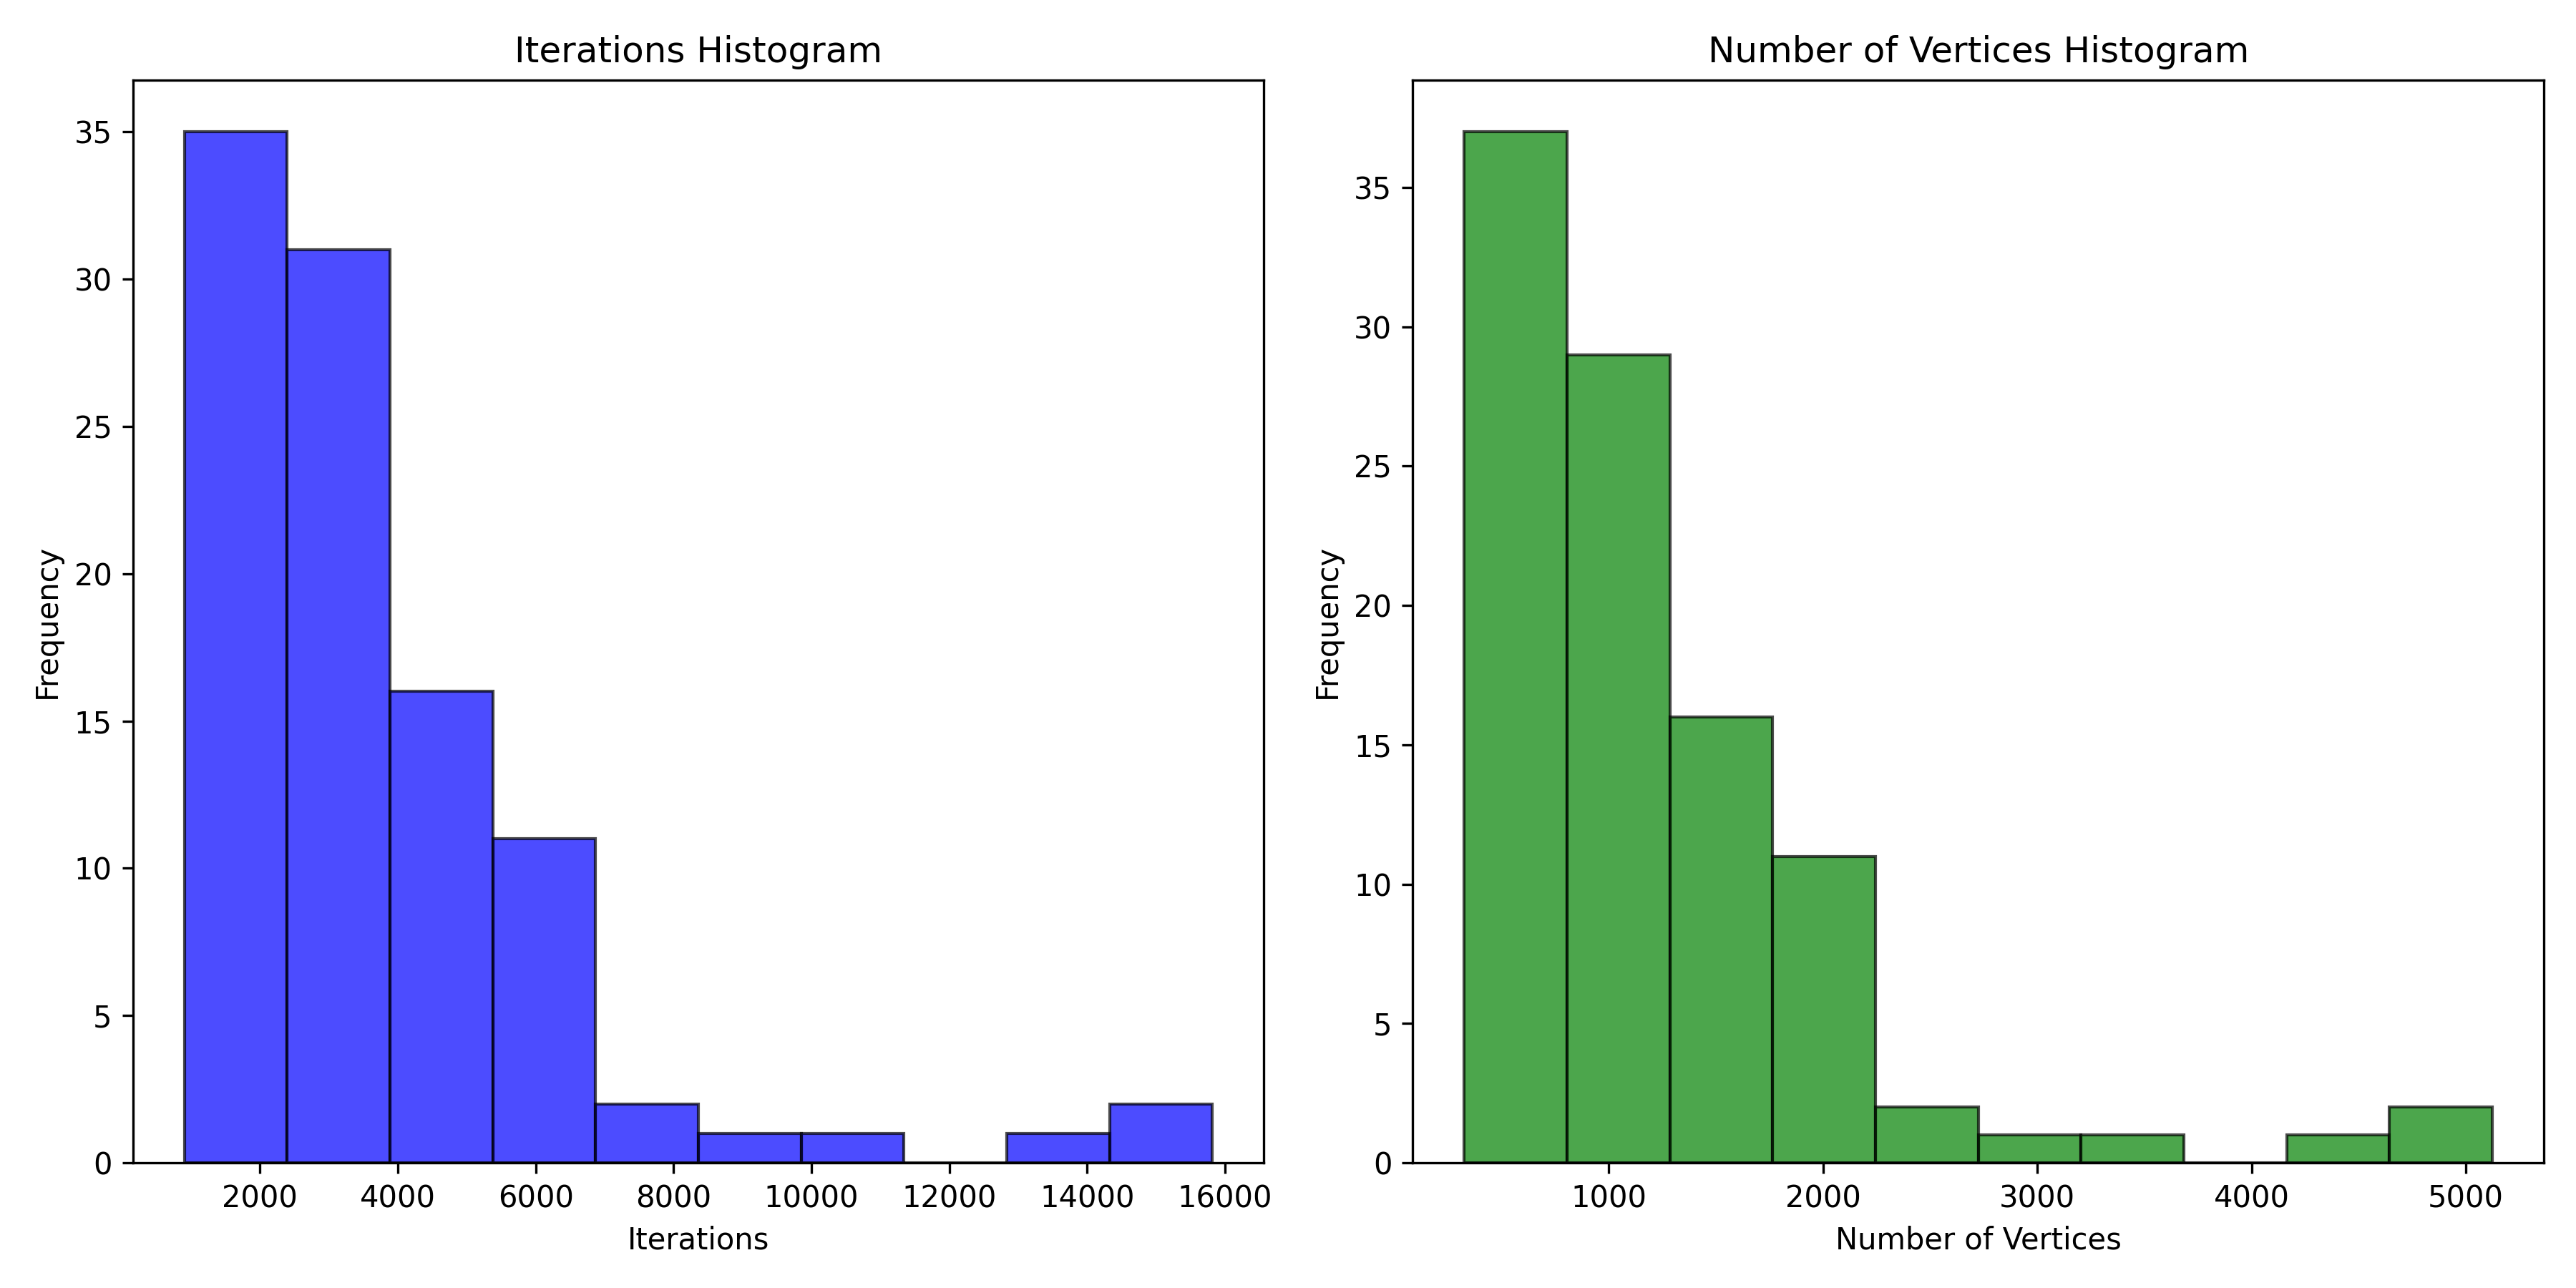
\includegraphics[width=0.65\textwidth]{figures/hist_RRT_Connect_4.png}
    \end{center}
    \caption{Histogram depicting number of iterations and number of
    vertices of RRT Connect with bug trap encircling goal over 100
trials}\label{fig:hist_RRT_Connect_4}
\end{figure}
\begin{figure}[H]
    \begin{center}
        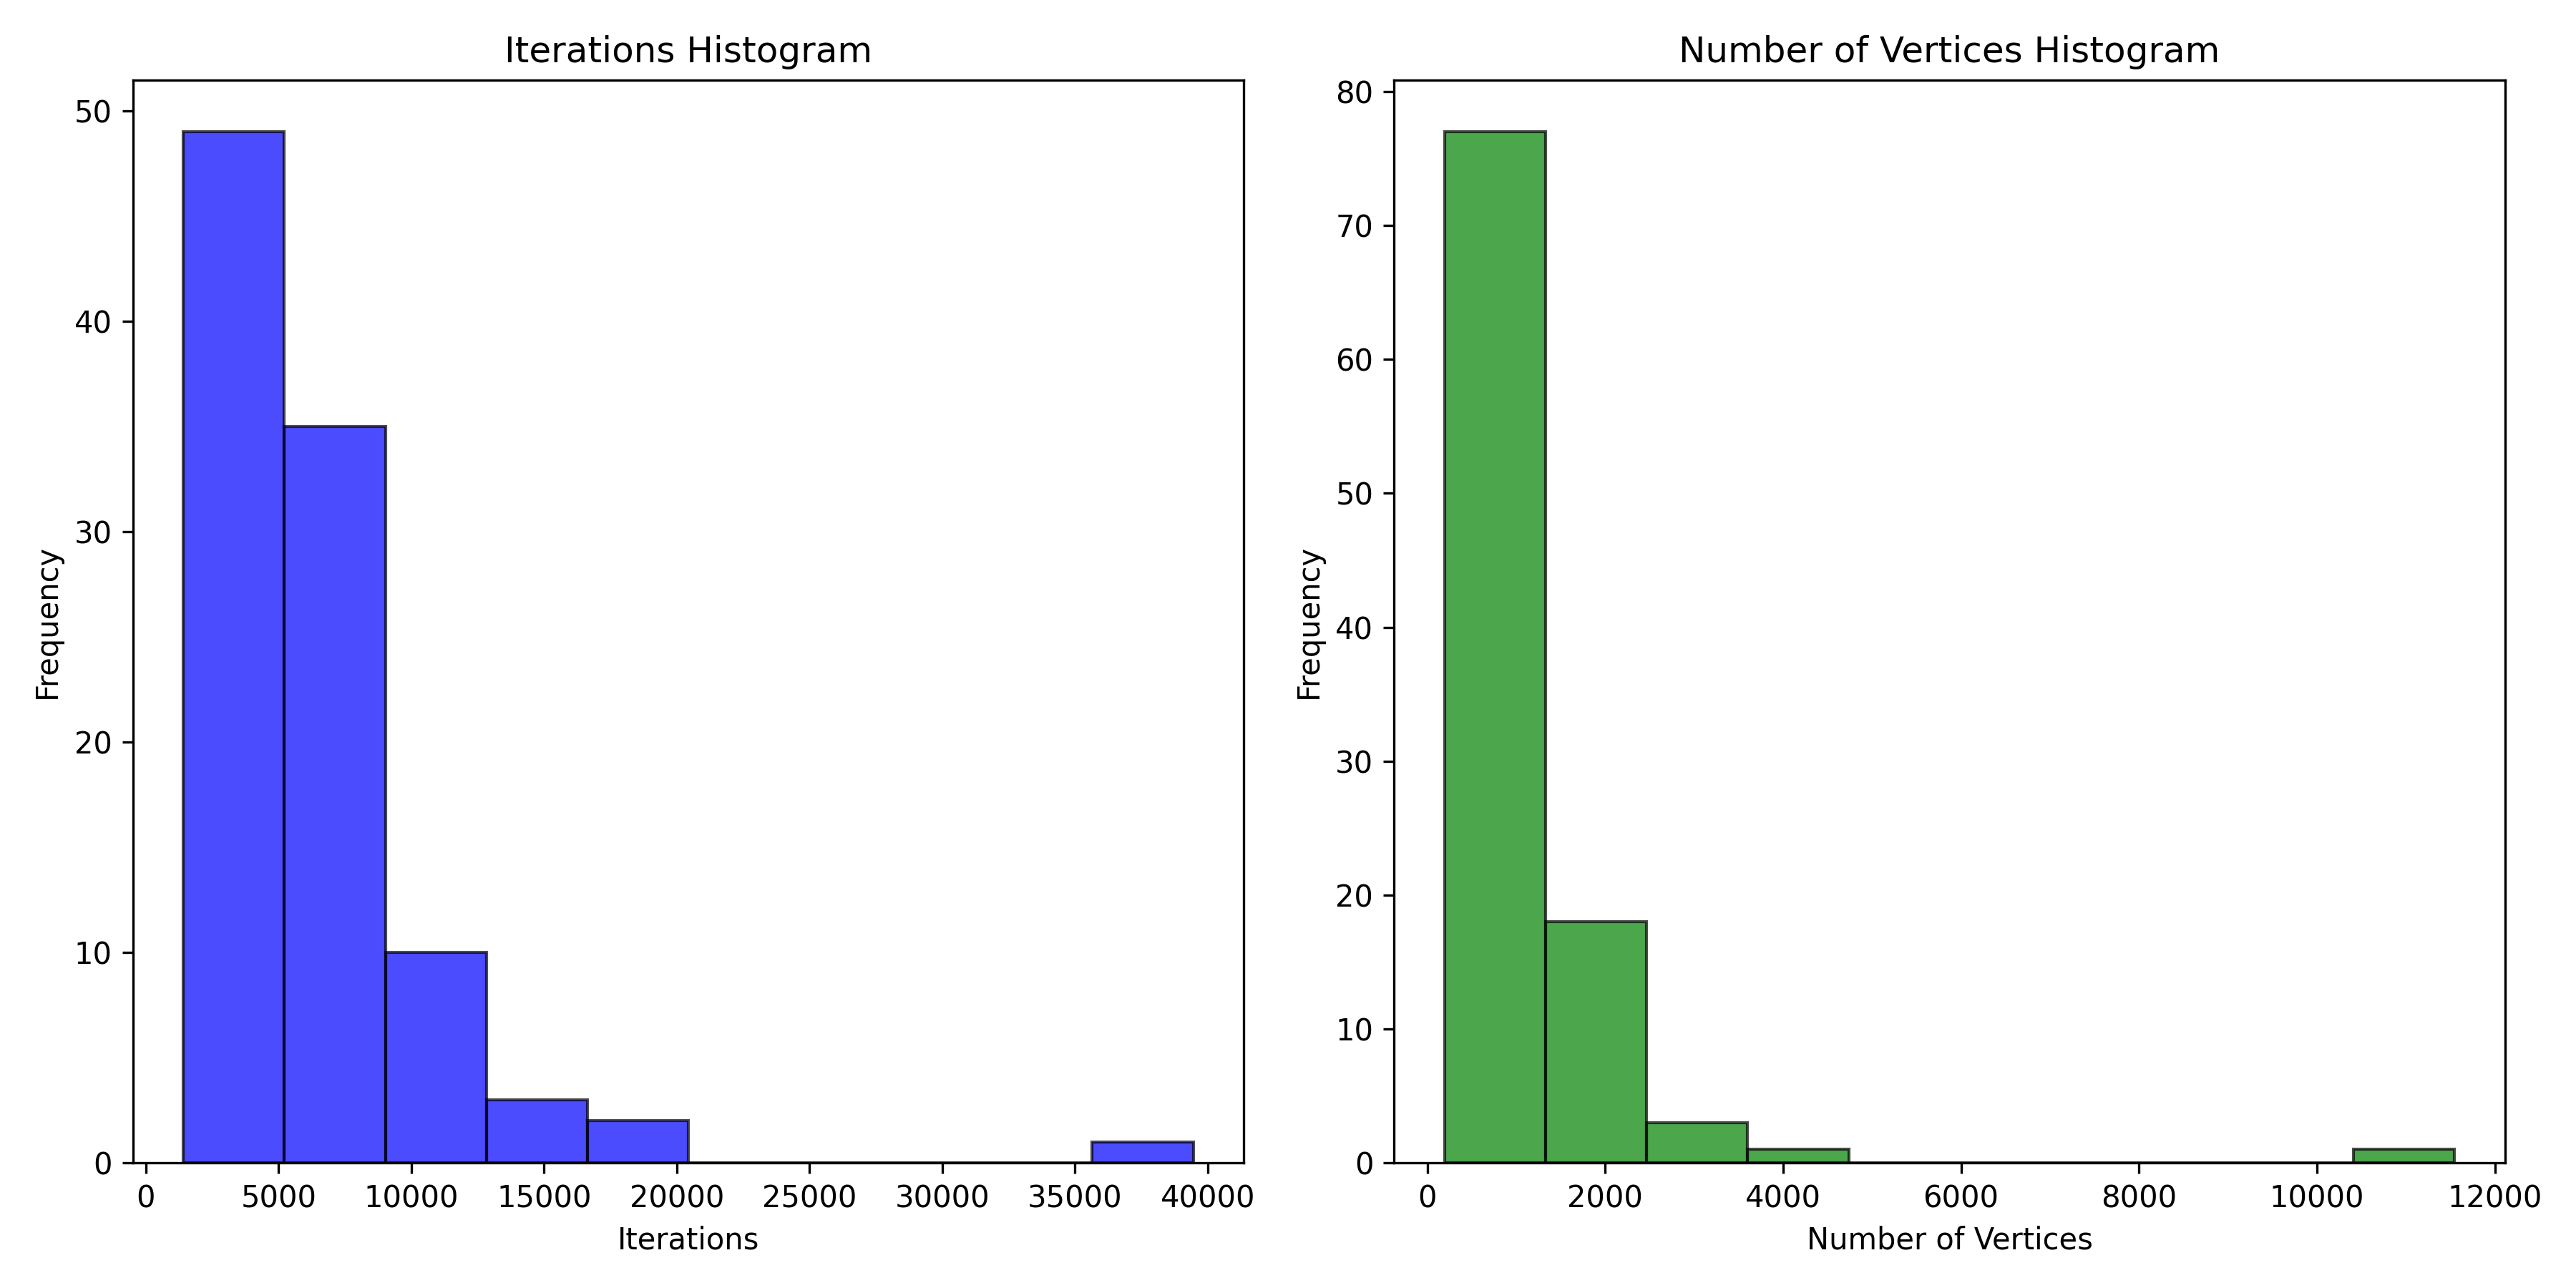
\includegraphics[width=0.65\textwidth]{figures/hist_RRT_Connect_5.png}
    \end{center}
    \caption{Histogram depicting number of iterations and number of
    vertices of RRT Connect with bug trap encircling start and goal over 100
trials}\label{fig:hist_RRT_Connect_5}
\end{figure}
% subsection Data and Figures 2 (end)

\subsection{Discussion}\label{sub:Discussion 2} % (fold)
\subsubsection{RRT}\label{sec:RRT} % (fold)
Looking at RRT first we observe a few interesting results. The first detail
of note is that it appears to have a smallest median path length when tested
on the world with enclosed goal. This in combination with the highest vertex
to iterations ratio of $0.91$ indicate it has no trouble expanding vertices,
but simply that it takes a long time (i.e. large number of iterations) to do,
supported by its higher median of iterations when compared the the enclosed start.
Figure \ref{fig:RRT_4} helps to support this qualitative observation as this 
example demonstrates the algorithm exhausting the non-enclosed region.
The enclosed start results indicate that algorithm has a very hard time leaving
enclosed region demonstrated through its low vertex/iteration ratio of $0.20$.
Looking at figure \ref{fig:RRT_3} we see that it generally fills the enclosed
region but upon escape it quickly and somewhat efficiently finds its way to the
goal. The doubly enclosed start and end see an approximate doubling in the 
median iterations which follows from the explanation given from above, the algorithm now
has to tackle the issue of escaping an enclosed region and entering into another.
An interesting statistic of note is that the vertex/iteration ratio here is at
$0.37$ which is a slight increase from the enclosed start. A possible explanation
to this "increase in efficiency" is perhaps not due to better performance but due to 
the same issue that arose with the enclosed goal experiment. Once the algorithm 
escaped the start it probably spent more time exhausting the un-enclosed region,
racking up "successful iterations" while in the case of the enclosed start, it
did not spend too much time in the unenclosed region as it quickly found a solution.
Another interesting statistic is from the fact that the median number of vertices
of the doubly enclosed start and goal was lower than the enclosed goal. This 
was probably caused by the simple fact that there is less free space to maneuver in
when compared to the enclosed goal.
% subsubsection RRT (end)
\subsubsection{RRT Connect}\label{sec:RRT Connect} % (fold)
As expected, RRT Connect performs somewhat similarly in both the enclosed start
and the enclosed goal cases. Both experience approximately the same
vertex/iteration ratio at $0.33$ and the median iterations and median vertices
also resemble each other closely. Finally, referring to their histograms 
(\ref{fig:hist_RRT_Connect_3})-(\ref{fig:hist_RRT_Connect_4}) also shows their
overwhelming similarilty.
Inspecting the doubly enclosed start and goal maps show a decrease in the 
vertex/iteration ratio at $0.15$ and an approximate $80\%$ increase in the 
median iterations but with a $20\%$ decrease in median vertices. This is probably
due to similar reasons as in the case of RRT.
% subsubsection RRT Connect (end)

\subsubsection{Comparing the two}\label{sec:Comparing the two} % (fold)
Comparing the two yields interesting observations. First we see that RRT 
usually requires fewer iterations to find a solution, this could be due to me 
incorrectly logging the iterations but it could also be due to some inherent 
inefficiency introduced by the connect function that I'm not very sure what it
could be. We also see that RRT Connect has more consistent vertex expansion between 
map types whereas RRT's vertex expansion total really depends on the conditions 
of its starting and ending position. The path length between the two seem to be similar
enough to assume that both algorithms find the same length solutions on average.
% subsubsection Comparing the two (end)

% subsection Discussion 2 (end)
	
\subsection{Code}\label{sub:Code 2} % (fold)
\subsubsection{RRT\_Connect.py}
\begin{minted}{python}
import random
from RRT import RRT, Vertex
from itertools import count

import matplotlib.pyplot as plt

class RRT_Connect(RRT):
    def __init__(self, start, goal, obstacle, workspace, animation=True, eta=2.5,
                 goal_sample_rate=0.01):
        super().__init__(start,goal,obstacle,workspace, animation, eta, goal_sample_rate)
        self.vertices_b = []

    def update_graph(self, sampled_vec=None):
        plt.clf()
        # Plot the sampled vector as a black plus sign
        if sampled_vec is not None:
            plt.plot(sampled_vec.x, sampled_vec.y, "Pk")

        # Plot edges as yellow lines
        for vertex in self.vertices:
            if vertex.parent:
                plt.plot(vertex.path_x, vertex.path_y, "-y")

        for vertex in self.vertices_b:
            if vertex.parent:
                plt.plot(vertex.path_x, vertex.path_y, "-y")

        for o in self.obstacle:
            # Plot the blue rectangle obstacle
            self.plot_rectangle(o)

        # Plot the green start "S" and red goal "G"
        plt.plot(self.start.x, self.start.y, c="g", marker=r"$\mathbb{S}$")
        plt.plot(self.goal.x, self.goal.y, c="r", marker=r"$\mathbb{G}$")

        plt.axis("equal")
        plt.axis([self.min_rand, self.max_rand, self.min_rand, self.max_rand])
        plt.grid(True)
        plt.pause(0.01)

    def planning(self):
        self.vertices = [self.start]
        self.vertices_b = [self.goal]
        for counter in count():  
            intersection = list(set(self.vertices).intersection(set(self.vertices_b)))
            if not len(intersection) == 0:
                self.iterations += counter
                break
            x_rand = self.sample_random_vertex()
            v_nearest = self.get_nearest_vertex(x_rand, self.vertices)
            x_new = self.steer(v_nearest, x_rand)

            if self.is_edge_valid(v_nearest, x_new):
                self.vertices.append(x_new)
                self.connect(x_new)

            if counter % 3 and self.animation is True == 0:
                self.update_graph(x_rand)

            self.vertices, self.vertices_b = self.vertices_b, self.vertices

        return self.final_paths(len(self.vertices) - 1, len(self.vertices_b) - 1)

    def connect(self, x_connect):
        v_nearest = self.get_nearest_vertex(x_connect, self.vertices_b)
        while True:
            x_step = self.steer(v_nearest, x_connect)
            if self.is_edge_valid(v_nearest, x_step):
                self.vertices_b.append(x_step)
                v_nearest = x_step

            self.iterations += 1
            if not (x_step != x_connect and self.is_edge_valid(v_nearest, x_step)):
                break
        return

    def final_paths(self, intersection_1, intersection_2):
        intersection = list(set(self.vertices).intersection(set(self.vertices_b)))
        if len(intersection) == 0:
            print("Error in breaking out of planning, the two sets do not share a vertex")

        path_a = [[intersection[0].x, intersection[0].y]]
        path_b = [[intersection[0].x, intersection[0].y]]

        vertex = self.vertices[intersection_1]
        while vertex.parent is not None:
            path_a.append([vertex.x, vertex.y])
            vertex = vertex.parent

        vertex_b = self.vertices_b[intersection_2]
        while vertex_b.parent is not None:
            path_b.append([vertex_b.x, vertex_b.y])
            vertex_b = vertex_b.parent

        path_a.append([vertex.x, vertex.y])
        path_b.append([vertex_b.x, vertex_b.y])
        path = path_a[1:][::-1] + path_b 
        self.num_vertices = len(self.vertices) + len(self.vertices_b)

        return path

    def sample_random_vertex(self):
        while True:
            sampled_vec = Vertex(random.uniform(self.min_rand, self.max_rand),
                random.uniform(self.min_rand, self.max_rand))
            if self.is_vertex_valid(sampled_vec):
                break
        return sampled_vec

\end{minted}
% subsection Code 2 (end)

\end{document}

